% Options for packages loaded elsewhere
% Options for packages loaded elsewhere
\PassOptionsToPackage{unicode}{hyperref}
\PassOptionsToPackage{hyphens}{url}
\PassOptionsToPackage{dvipsnames,svgnames,x11names}{xcolor}
%
\documentclass[
  letterpaper,
  DIV=11,
  numbers=noendperiod,
  oneside]{scrartcl}
\usepackage{xcolor}
\usepackage[left=1in,marginparwidth=2.0666666666667in,textwidth=4.1333333333333in,marginparsep=0.3in]{geometry}
\usepackage{amsmath,amssymb}
\setcounter{secnumdepth}{-\maxdimen} % remove section numbering
\usepackage{iftex}
\ifPDFTeX
  \usepackage[T1]{fontenc}
  \usepackage[utf8]{inputenc}
  \usepackage{textcomp} % provide euro and other symbols
\else % if luatex or xetex
  \usepackage{unicode-math} % this also loads fontspec
  \defaultfontfeatures{Scale=MatchLowercase}
  \defaultfontfeatures[\rmfamily]{Ligatures=TeX,Scale=1}
\fi
\usepackage{lmodern}
\ifPDFTeX\else
  % xetex/luatex font selection
\fi
% Use upquote if available, for straight quotes in verbatim environments
\IfFileExists{upquote.sty}{\usepackage{upquote}}{}
\IfFileExists{microtype.sty}{% use microtype if available
  \usepackage[]{microtype}
  \UseMicrotypeSet[protrusion]{basicmath} % disable protrusion for tt fonts
}{}
\makeatletter
\@ifundefined{KOMAClassName}{% if non-KOMA class
  \IfFileExists{parskip.sty}{%
    \usepackage{parskip}
  }{% else
    \setlength{\parindent}{0pt}
    \setlength{\parskip}{6pt plus 2pt minus 1pt}}
}{% if KOMA class
  \KOMAoptions{parskip=half}}
\makeatother
% Make \paragraph and \subparagraph free-standing
\makeatletter
\ifx\paragraph\undefined\else
  \let\oldparagraph\paragraph
  \renewcommand{\paragraph}{
    \@ifstar
      \xxxParagraphStar
      \xxxParagraphNoStar
  }
  \newcommand{\xxxParagraphStar}[1]{\oldparagraph*{#1}\mbox{}}
  \newcommand{\xxxParagraphNoStar}[1]{\oldparagraph{#1}\mbox{}}
\fi
\ifx\subparagraph\undefined\else
  \let\oldsubparagraph\subparagraph
  \renewcommand{\subparagraph}{
    \@ifstar
      \xxxSubParagraphStar
      \xxxSubParagraphNoStar
  }
  \newcommand{\xxxSubParagraphStar}[1]{\oldsubparagraph*{#1}\mbox{}}
  \newcommand{\xxxSubParagraphNoStar}[1]{\oldsubparagraph{#1}\mbox{}}
\fi
\makeatother

\usepackage{color}
\usepackage{fancyvrb}
\newcommand{\VerbBar}{|}
\newcommand{\VERB}{\Verb[commandchars=\\\{\}]}
\DefineVerbatimEnvironment{Highlighting}{Verbatim}{commandchars=\\\{\}}
% Add ',fontsize=\small' for more characters per line
\usepackage{framed}
\definecolor{shadecolor}{RGB}{241,243,245}
\newenvironment{Shaded}{\begin{snugshade}}{\end{snugshade}}
\newcommand{\AlertTok}[1]{\textcolor[rgb]{0.68,0.00,0.00}{#1}}
\newcommand{\AnnotationTok}[1]{\textcolor[rgb]{0.37,0.37,0.37}{#1}}
\newcommand{\AttributeTok}[1]{\textcolor[rgb]{0.40,0.45,0.13}{#1}}
\newcommand{\BaseNTok}[1]{\textcolor[rgb]{0.68,0.00,0.00}{#1}}
\newcommand{\BuiltInTok}[1]{\textcolor[rgb]{0.00,0.23,0.31}{#1}}
\newcommand{\CharTok}[1]{\textcolor[rgb]{0.13,0.47,0.30}{#1}}
\newcommand{\CommentTok}[1]{\textcolor[rgb]{0.37,0.37,0.37}{#1}}
\newcommand{\CommentVarTok}[1]{\textcolor[rgb]{0.37,0.37,0.37}{\textit{#1}}}
\newcommand{\ConstantTok}[1]{\textcolor[rgb]{0.56,0.35,0.01}{#1}}
\newcommand{\ControlFlowTok}[1]{\textcolor[rgb]{0.00,0.23,0.31}{\textbf{#1}}}
\newcommand{\DataTypeTok}[1]{\textcolor[rgb]{0.68,0.00,0.00}{#1}}
\newcommand{\DecValTok}[1]{\textcolor[rgb]{0.68,0.00,0.00}{#1}}
\newcommand{\DocumentationTok}[1]{\textcolor[rgb]{0.37,0.37,0.37}{\textit{#1}}}
\newcommand{\ErrorTok}[1]{\textcolor[rgb]{0.68,0.00,0.00}{#1}}
\newcommand{\ExtensionTok}[1]{\textcolor[rgb]{0.00,0.23,0.31}{#1}}
\newcommand{\FloatTok}[1]{\textcolor[rgb]{0.68,0.00,0.00}{#1}}
\newcommand{\FunctionTok}[1]{\textcolor[rgb]{0.28,0.35,0.67}{#1}}
\newcommand{\ImportTok}[1]{\textcolor[rgb]{0.00,0.46,0.62}{#1}}
\newcommand{\InformationTok}[1]{\textcolor[rgb]{0.37,0.37,0.37}{#1}}
\newcommand{\KeywordTok}[1]{\textcolor[rgb]{0.00,0.23,0.31}{\textbf{#1}}}
\newcommand{\NormalTok}[1]{\textcolor[rgb]{0.00,0.23,0.31}{#1}}
\newcommand{\OperatorTok}[1]{\textcolor[rgb]{0.37,0.37,0.37}{#1}}
\newcommand{\OtherTok}[1]{\textcolor[rgb]{0.00,0.23,0.31}{#1}}
\newcommand{\PreprocessorTok}[1]{\textcolor[rgb]{0.68,0.00,0.00}{#1}}
\newcommand{\RegionMarkerTok}[1]{\textcolor[rgb]{0.00,0.23,0.31}{#1}}
\newcommand{\SpecialCharTok}[1]{\textcolor[rgb]{0.37,0.37,0.37}{#1}}
\newcommand{\SpecialStringTok}[1]{\textcolor[rgb]{0.13,0.47,0.30}{#1}}
\newcommand{\StringTok}[1]{\textcolor[rgb]{0.13,0.47,0.30}{#1}}
\newcommand{\VariableTok}[1]{\textcolor[rgb]{0.07,0.07,0.07}{#1}}
\newcommand{\VerbatimStringTok}[1]{\textcolor[rgb]{0.13,0.47,0.30}{#1}}
\newcommand{\WarningTok}[1]{\textcolor[rgb]{0.37,0.37,0.37}{\textit{#1}}}

\usepackage{longtable,booktabs,array}
\usepackage{calc} % for calculating minipage widths
% Correct order of tables after \paragraph or \subparagraph
\usepackage{etoolbox}
\makeatletter
\patchcmd\longtable{\par}{\if@noskipsec\mbox{}\fi\par}{}{}
\makeatother
% Allow footnotes in longtable head/foot
\IfFileExists{footnotehyper.sty}{\usepackage{footnotehyper}}{\usepackage{footnote}}
\makesavenoteenv{longtable}
\usepackage{graphicx}
\makeatletter
\newsavebox\pandoc@box
\newcommand*\pandocbounded[1]{% scales image to fit in text height/width
  \sbox\pandoc@box{#1}%
  \Gscale@div\@tempa{\textheight}{\dimexpr\ht\pandoc@box+\dp\pandoc@box\relax}%
  \Gscale@div\@tempb{\linewidth}{\wd\pandoc@box}%
  \ifdim\@tempb\p@<\@tempa\p@\let\@tempa\@tempb\fi% select the smaller of both
  \ifdim\@tempa\p@<\p@\scalebox{\@tempa}{\usebox\pandoc@box}%
  \else\usebox{\pandoc@box}%
  \fi%
}
% Set default figure placement to htbp
\def\fps@figure{htbp}
\makeatother





\setlength{\emergencystretch}{3em} % prevent overfull lines

\providecommand{\tightlist}{%
  \setlength{\itemsep}{0pt}\setlength{\parskip}{0pt}}



 


\KOMAoption{captions}{tableheading}
\makeatletter
\@ifpackageloaded{tcolorbox}{}{\usepackage[skins,breakable]{tcolorbox}}
\@ifpackageloaded{fontawesome5}{}{\usepackage{fontawesome5}}
\definecolor{quarto-callout-color}{HTML}{909090}
\definecolor{quarto-callout-note-color}{HTML}{0758E5}
\definecolor{quarto-callout-important-color}{HTML}{CC1914}
\definecolor{quarto-callout-warning-color}{HTML}{EB9113}
\definecolor{quarto-callout-tip-color}{HTML}{00A047}
\definecolor{quarto-callout-caution-color}{HTML}{FC5300}
\definecolor{quarto-callout-color-frame}{HTML}{acacac}
\definecolor{quarto-callout-note-color-frame}{HTML}{4582ec}
\definecolor{quarto-callout-important-color-frame}{HTML}{d9534f}
\definecolor{quarto-callout-warning-color-frame}{HTML}{f0ad4e}
\definecolor{quarto-callout-tip-color-frame}{HTML}{02b875}
\definecolor{quarto-callout-caution-color-frame}{HTML}{fd7e14}
\makeatother
\makeatletter
\@ifpackageloaded{caption}{}{\usepackage{caption}}
\AtBeginDocument{%
\ifdefined\contentsname
  \renewcommand*\contentsname{Table of contents}
\else
  \newcommand\contentsname{Table of contents}
\fi
\ifdefined\listfigurename
  \renewcommand*\listfigurename{List of Figures}
\else
  \newcommand\listfigurename{List of Figures}
\fi
\ifdefined\listtablename
  \renewcommand*\listtablename{List of Tables}
\else
  \newcommand\listtablename{List of Tables}
\fi
\ifdefined\figurename
  \renewcommand*\figurename{Figure}
\else
  \newcommand\figurename{Figure}
\fi
\ifdefined\tablename
  \renewcommand*\tablename{Table}
\else
  \newcommand\tablename{Table}
\fi
}
\@ifpackageloaded{float}{}{\usepackage{float}}
\floatstyle{ruled}
\@ifundefined{c@chapter}{\newfloat{codelisting}{h}{lop}}{\newfloat{codelisting}{h}{lop}[chapter]}
\floatname{codelisting}{Listing}
\newcommand*\listoflistings{\listof{codelisting}{List of Listings}}
\makeatother
\makeatletter
\makeatother
\makeatletter
\@ifpackageloaded{caption}{}{\usepackage{caption}}
\@ifpackageloaded{subcaption}{}{\usepackage{subcaption}}
\makeatother
\makeatletter
\@ifpackageloaded{sidenotes}{}{\usepackage{sidenotes}}
\@ifpackageloaded{marginnote}{}{\usepackage{marginnote}}
\makeatother
\usepackage{bookmark}
\IfFileExists{xurl.sty}{\usepackage{xurl}}{} % add URL line breaks if available
\urlstyle{same}
\hypersetup{
  colorlinks=true,
  linkcolor={blue},
  filecolor={Maroon},
  citecolor={Blue},
  urlcolor={Blue},
  pdfcreator={LaTeX via pandoc}}


\author{}
\date{}
\begin{document}


\subsection{Title Slide}\label{title-slide}

Discrete-Time Control Design 3

Optimal Control

Dr Guilherme Froes Silva School of Electrical Engineering \& Robotics
Queensland University of Technology

EGH445 - Modern Control

Consultation: GP-S1111 Email: g.froessilva@qut.edu.au

\section{Overview}\label{overview}

\begin{itemize}
\tightlist
\item
  Quick review of (some of) the content so far.
\item
  When does pole placement work well? {And when does it fail?}
\item
  What is \emph{Optimal} Control?
\item
  Why should we do optimal control instead of just pole placement?
\item
  The Optimal Control Problem.
\item
  The Linear Quadratic Regulator (LQR).
\item
  Model Predictive Control (MPC).
\end{itemize}

\subsection{Quick review of (some of) the content so
far}\label{quick-review-of-some-of-the-content-so-far}

. . .

\textbf{Continuous-time system:} \[ 
\begin{align*}\dot{x}(t) &= f(x, u), \\ y(t) &= g(x, u) \end{align*} 
\]

. . .

\textbf{Linearised system:} \[ 
\begin{align*} 
\delta\dot{x}(t) &= A\delta x(t) + B \delta u(t),  \\ 
\delta y(t) &= C\delta x(t) + D\delta u(t),
\end{align*} 
\]

where \(\delta x = x - \bar x\), \(\delta u = u - \bar u\),
\(\delta y = y - \bar y\), and the \(A\), \(B\), \(C\), \(D\) are the
matrices \[ 
\begin{align*}
A = \frac{\partial f}{\partial x} \bigg|_{\bar x, \bar u}
B = \frac{\partial f}{\partial u} \bigg|_{\bar x, \bar u}
C = \frac{\partial g}{\partial x} \bigg|_{\bar x, \bar u}
D = \frac{\partial g}{\partial u} \bigg|_{\bar x, \bar u} 
\end{align*}
\]

. . .

\textbf{Discrete-time system:} \[
\begin{align*} x(kT+T) &= Gx(kT) + Hu(kT), \\ y(kT) &= Cx(kT) + Du(kT), \end{align*}
\]

where \[
\begin{align*}
G = e^{AT}, \quad H = \left[\int_0^T e^{A\tau} d\tau\right] B \quad \left(\text{or, if $A$ is invertible, } H = A^{-1} (G-I)B\right)
\end{align*}
\]

. . .

\textbf{State-feedback controller:} \[ 
\begin{align*}
u(k) = -Kx(kT) 
\end{align*}
\]

where \(K\) is the feedback gain matrix that is designed to arbitrarily
move the poles of the closed-loop system \[
\begin{align*}
x(kT+T) = (G-HK)x(kT)
\end{align*}
\]

for example, by equating the characteristic polynomial of the
closed-loop system to a desired polynomial, \[
\begin{align*}
\det(zI - (G-HK)) = (z - z_1)(z - z_2) \cdots (z - z_n) 
\end{align*}
\]

. . .

\begin{tcolorbox}[enhanced jigsaw, rightrule=.15mm, coltitle=black, titlerule=0mm, breakable, title=\textcolor{quarto-callout-important-color}{\faExclamation}\hspace{0.5em}{Important}, bottomrule=.15mm, colback=white, toprule=.15mm, opacityback=0, opacitybacktitle=0.6, leftrule=.75mm, left=2mm, colbacktitle=quarto-callout-important-color!10!white, bottomtitle=1mm, toptitle=1mm, arc=.35mm, colframe=quarto-callout-important-color-frame]

The solution exists if the system is controllable, i.e.~if the
\textbf{controllability matrix}
\(\;\mathcal{C} = \left[H,\; GH,\; G^2H,\; \ldots,\; G^{n-1}H\right]\)
has full rank (\(\text{rank}(\mathcal{C})=n\)).

\end{tcolorbox}

. . .

\textbf{How do you choose the poles?}

\begin{itemize}
\tightlist
\item
  \(t_s\) - settling time
\item
  \(t_r\) - rise time
\item
  \(\%OS\) - percent overshoot
\item
  \(\omega_n\) - natural frequency
\item
  \(\zeta\) - damping ratio (or through percent overshoot)
\end{itemize}

\begin{itemize}
\tightlist
\item
  \(\zeta = \dfrac{\ln(\%OS/100)}{\sqrt{\pi^2 + \ln^2(\%OS/100)}}\)
\item
  \(\omega_n = \frac{4}{\zeta t_s}\)
\item
  \(s_{1,2} = -\zeta \omega_n \pm j \omega_n \sqrt{1-\zeta^2}\)
\item
  \(z_{1,2} = e^{s_{1,2}T}\)
\end{itemize}

. . .

We also saw the \textbf{Internal Model Principle} (e.g.~\textbf{Integral
Action}) to reject disturbances (or follow references) with a known
model (e.g.~a step input, a ramp input, a sinusoidal input, etc.). Those
still relied on the \textbf{pole placement} approach.

\section{Limitations of Pole
placement}\label{limitations-of-pole-placement}

. . .

\emph{Works well for:}

\begin{itemize}
\tightlist
\item
  SISO systems (Single Input Single Output)
\item
  Low order systems (2nd order or when 2nd order \emph{dominant}, etc.)
\end{itemize}

. . .

\emph{Does not work well for:}

\begin{itemize}
\tightlist
\item
  \textbf{Higher-order systems} (4th order, 5th order, etc.)
\item
  \textbf{MIMO systems} (Multiple Input Multiple Output)
\item
  \emph{Stiff} systems (e.g.~with very different time constants,
  e.g.~1ms and 1s)
\item
  \textbf{Highly nonlinear systems} (i.e.~when the linearisation quickly
  becomes invalid.)
\end{itemize}

\subsection{Higher-Order Systems}\label{higher-order-systems}

\[
\begin{align*} x(kT+T) &= Gx(kT) + Hu(kT), \\ y(kT) &= Cx(kT) + Du(kT), \end{align*}
\]

where
\(\quad x(kT) \in \mathbb{R}^n, \quad u(kT) \in \mathbb{R}, \quad y(kT) \in \mathbb{R}, \quad n > 3\)

. . .

\begin{tcolorbox}[enhanced jigsaw, rightrule=.15mm, coltitle=black, titlerule=0mm, breakable, title=\textcolor{quarto-callout-important-color}{\faExclamation}\hspace{0.5em}{Important}, bottomrule=.15mm, colback=white, toprule=.15mm, opacityback=0, opacitybacktitle=0.6, leftrule=.75mm, left=2mm, colbacktitle=quarto-callout-important-color!10!white, bottomtitle=1mm, toptitle=1mm, arc=.35mm, colframe=quarto-callout-important-color-frame]

The link between pole locations and desired time-domain response becomes
less clear. Arbitrary choices can lead to poor performance or excessive
control effort.

\emph{How do you choose the best pole locations for a 5th, 10th, or
higher-order system?}

\end{tcolorbox}

\subsection{MIMO Systems}\label{mimo-systems}

Let's start with an example.

Consider a simple MIMO system with two states and two inputs: \[
\begin{align*} x(kT+T) &= \begin{bmatrix} 1 & 0.1 \\ 0 & 0.8 \end{bmatrix} x(kT) + \begin{bmatrix} 1 & 0 \\ 0 & 1 \end{bmatrix} u(kT)
\end{align*} 
\]

We want to place the poles at \(0.4\) and \(0.6\), by using
\(u(kT) = -Kx(kT)\), where
\(K = \begin{bmatrix} k_1 & k_2 \\ k_3 & k_4\end{bmatrix}\).

. . .

The characteristic polynomial is given by: \[
\begin{align*}
&\det(zI - (G-HK)) = \det\left(\begin{bmatrix} z-1+k_1 & k_2-0.1 \\ k_3 & z-0.8+k_4\end{bmatrix}\right) \\
&= z^2 + (k_1 + k_4 - 1.8)z + (0.1k_3 - k_4 - 0.8k_1 + k_1k_4 - k_2k_3 + 0.8)
\end{align*}
\]

. . .

The desired characteristic polynomial is given by: \[
\begin{align*}
(z-0.4)(z-0.6) = z^2 - 1z + 0.24
\end{align*}
\]

. . .

When we equate the coefficients, we get: \[
\begin{align*}
\begin{cases}
(k_1 + k_4 - 1.8) = -1 \\
0.1k_3 - k_4 - 0.8k_1 + k_1k_4 - k_2k_3 + 0.8 = 0.24
\end{cases}
\end{align*}
\]

. . .

\begin{tcolorbox}[enhanced jigsaw, rightrule=.15mm, coltitle=black, titlerule=0mm, breakable, title=\textcolor{quarto-callout-important-color}{\faExclamation}\hspace{0.5em}{Important}, bottomrule=.15mm, colback=white, toprule=.15mm, opacityback=0, opacitybacktitle=0.6, leftrule=.75mm, left=2mm, colbacktitle=quarto-callout-important-color!10!white, bottomtitle=1mm, toptitle=1mm, arc=.35mm, colframe=quarto-callout-important-color-frame]

Note that we have \textbf{two equations} and \textbf{four unknowns}.
This means that we have \textbf{degrees of freedom} in the design. We
can choose two of the four variables arbitrarily, and then solve for the
other two.

\end{tcolorbox}

. . .

This seems like a good idea, but it is not. The problem is that
different choices of \(K\), even if they lead to the same
\textbf{eigenvalues}, can lead to different \textbf{eigenvectors}. The
closed-loop system's \textbf{eigenvectors} directly affect the
\textbf{response} of the system.

. . .

Let \(k_2 = k_3 = 0\) and consider the following two cases of gains
matrices \(K_1\) and \(K_2\), both of which lead assign the closed-loop
eigenvalues to the desired values: \[
K_1 = \begin{bmatrix} 0.6 & 0 \\ 0 & 0.2 \end{bmatrix}, \quad K_2 = \begin{bmatrix} 0.4 & 0 \\ 0 & 0.4 \end{bmatrix}
\]

Both of which lead to the same eigenvalues we wanted. But let's simulate
the system with both \(K_1\) and \(K_2\).

\begin{Shaded}
\begin{Highlighting}[numbers=left,,]
\ImportTok{import}\NormalTok{ numpy }\ImportTok{as}\NormalTok{ np}
\ImportTok{import}\NormalTok{ matplotlib.pyplot }\ImportTok{as}\NormalTok{ plt}
\ImportTok{import}\NormalTok{ control }\ImportTok{as}\NormalTok{ ctrl}
\CommentTok{\# Create the system matrices}
\NormalTok{G }\OperatorTok{=}\NormalTok{ np.array([[}\DecValTok{1}\NormalTok{, }\FloatTok{0.1}\NormalTok{], [}\DecValTok{0}\NormalTok{, }\FloatTok{0.8}\NormalTok{]])}
\NormalTok{H }\OperatorTok{=}\NormalTok{ np.array([[}\DecValTok{1}\NormalTok{, }\DecValTok{0}\NormalTok{], [}\DecValTok{0}\NormalTok{, }\DecValTok{1}\NormalTok{]])}
\NormalTok{C }\OperatorTok{=}\NormalTok{ np.array([[}\DecValTok{1}\NormalTok{, }\DecValTok{0}\NormalTok{], [}\DecValTok{0}\NormalTok{, }\DecValTok{1}\NormalTok{]]) }\CommentTok{\# Outputs are the states}
\NormalTok{D }\OperatorTok{=}\NormalTok{ np.array([[}\DecValTok{0}\NormalTok{, }\DecValTok{0}\NormalTok{], [}\DecValTok{0}\NormalTok{, }\DecValTok{0}\NormalTok{]])}
\NormalTok{K1 }\OperatorTok{=}\NormalTok{ np.array([[}\FloatTok{0.6}\NormalTok{, }\DecValTok{0}\NormalTok{], [}\DecValTok{0}\NormalTok{, }\FloatTok{0.2}\NormalTok{]]) }
\NormalTok{K2 }\OperatorTok{=}\NormalTok{ np.array([[}\FloatTok{0.4}\NormalTok{, }\DecValTok{0}\NormalTok{], [}\DecValTok{0}\NormalTok{, }\FloatTok{0.4}\NormalTok{]]) }
\NormalTok{Gcl1 }\OperatorTok{=}\NormalTok{ G }\OperatorTok{{-}}\NormalTok{ H }\OperatorTok{@}\NormalTok{ K1 }
\NormalTok{Gcl2 }\OperatorTok{=}\NormalTok{ G }\OperatorTok{{-}}\NormalTok{ H }\OperatorTok{@}\NormalTok{ K2}

\NormalTok{Ts }\OperatorTok{=} \FloatTok{0.1} \CommentTok{\# Sampling time (seconds)}
\CommentTok{\# Create the closed{-}loop LTI systems}
\NormalTok{sys1 }\OperatorTok{=}\NormalTok{ ctrl.ss(Gcl1, H, C, D, Ts) }
\NormalTok{sys2 }\OperatorTok{=}\NormalTok{ ctrl.ss(Gcl2, H, C, D, Ts) }

\CommentTok{\# Simulate for initial condition x0 = [1, 0]}
\NormalTok{x0 }\OperatorTok{=}\NormalTok{ np.array([}\DecValTok{1}\NormalTok{, }\DecValTok{0}\NormalTok{])}
\NormalTok{t\_end }\OperatorTok{=} \FloatTok{1.5} 
\NormalTok{t }\OperatorTok{=}\NormalTok{ np.arange(}\DecValTok{0}\NormalTok{, t\_end, Ts) }
\NormalTok{t1, y1 }\OperatorTok{=}\NormalTok{ ctrl.initial\_response(sys1, T}\OperatorTok{=}\NormalTok{t, X0}\OperatorTok{=}\NormalTok{x0)}
\NormalTok{t2, y2 }\OperatorTok{=}\NormalTok{ ctrl.initial\_response(sys2, T}\OperatorTok{=}\NormalTok{t, X0}\OperatorTok{=}\NormalTok{x0)}

\NormalTok{plt.figure(figsize}\OperatorTok{=}\NormalTok{(}\DecValTok{10}\NormalTok{, }\DecValTok{8}\NormalTok{))}
\NormalTok{plt.plot(t1, y1[}\DecValTok{0}\NormalTok{, :], label}\OperatorTok{=}\StringTok{\textquotesingle{}K1 {-} x1\textquotesingle{}}\NormalTok{, linewidth}\OperatorTok{=}\DecValTok{3}\NormalTok{)}
\NormalTok{plt.plot(t1, y1[}\DecValTok{1}\NormalTok{, :], label}\OperatorTok{=}\StringTok{\textquotesingle{}K1 {-} x2\textquotesingle{}}\NormalTok{, linewidth}\OperatorTok{=}\DecValTok{3}\NormalTok{)}
\NormalTok{plt.plot(t2, y2[}\DecValTok{0}\NormalTok{, :], label}\OperatorTok{=}\StringTok{\textquotesingle{}K2 {-} x1\textquotesingle{}}\NormalTok{, linestyle}\OperatorTok{=}\StringTok{\textquotesingle{}{-}{-}\textquotesingle{}}\NormalTok{, linewidth}\OperatorTok{=}\DecValTok{3}\NormalTok{) }
\NormalTok{plt.plot(t2, y2[}\DecValTok{1}\NormalTok{, :], label}\OperatorTok{=}\StringTok{\textquotesingle{}K2 {-} x2\textquotesingle{}}\NormalTok{, linestyle}\OperatorTok{=}\StringTok{\textquotesingle{}{-}{-}\textquotesingle{}}\NormalTok{, linewidth}\OperatorTok{=}\DecValTok{3}\NormalTok{) }
\NormalTok{plt.title(}\StringTok{\textquotesingle{}Initial Condition Response ($x\_0=[1, 0]\^{}T$) with Different K Matrices\textquotesingle{}}\NormalTok{, fontsize}\OperatorTok{=}\DecValTok{16}\NormalTok{) }
\NormalTok{plt.xlabel(}\StringTok{\textquotesingle{}Time (steps * dt)\textquotesingle{}}\NormalTok{, fontsize}\OperatorTok{=}\DecValTok{14}\NormalTok{) }
\NormalTok{plt.ylabel(}\StringTok{\textquotesingle{}State Values\textquotesingle{}}\NormalTok{, fontsize}\OperatorTok{=}\DecValTok{14}\NormalTok{) }
\NormalTok{plt.legend(fontsize}\OperatorTok{=}\DecValTok{12}\NormalTok{)}
\NormalTok{plt.grid(}\VariableTok{True}\NormalTok{) }
\NormalTok{plt.show()}
\end{Highlighting}
\end{Shaded}

\pandocbounded{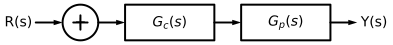
\includegraphics[keepaspectratio]{lecture9_files/figure-pdf/cell-2-output-1.png}}

\begin{center}\rule{0.5\linewidth}{0.5pt}\end{center}

\subsection{MIMO Systems}\label{mimo-systems-1}

\[
\begin{align*} x(kT+T) &= Gx(kT) + Hu(kT), \\ y(kT) &= Cx(kT) + Du(kT), \end{align*}
\]

\(x(kT) \in \mathbb{R}^n, \quad u(kT) \in \mathbb{R}^m, \quad y(kT) \in \mathbb{R}^p, \quad n, m, p > 1\)

. . .

\begin{tcolorbox}[enhanced jigsaw, rightrule=.15mm, coltitle=black, titlerule=0mm, breakable, title=\textcolor{quarto-callout-important-color}{\faExclamation}\hspace{0.5em}{Important}, bottomrule=.15mm, colback=white, toprule=.15mm, opacityback=0, opacitybacktitle=0.6, leftrule=.75mm, left=2mm, colbacktitle=quarto-callout-important-color!10!white, bottomtitle=1mm, toptitle=1mm, arc=.35mm, colframe=quarto-callout-important-color-frame]

For MIMO systems, pole placement is significantly more complex.
Specifying only the eigenvalues leaves \textbf{degrees of freedom} in
the \textbf{eigenvectors}, which also \textbf{affect the response}. The
design process becomes \textbf{non-unique} and less intuitive.

\emph{How do you systematically handle interactions between different
inputs and outputs?}

\end{tcolorbox}

\subsection{Performance trade-off}\label{performance-trade-off}

Finally, pole placement does not consider the \textbf{control effort},
not addressing the trade-off between:

\begin{itemize}
\item
  regulating the state, by making \(x(kT)\), or \(\delta x(kT)\)1, small

  1 For linearised systems, we defined \(\delta x = x - \bar x\).
\item
  \emph{regulating} required control effort \(u(kT)\).
\end{itemize}

. . .

\begin{tcolorbox}[enhanced jigsaw, rightrule=.15mm, coltitle=black, titlerule=0mm, breakable, title=\textcolor{quarto-callout-important-color}{\faExclamation}\hspace{0.5em}{Important}, bottomrule=.15mm, colback=white, toprule=.15mm, opacityback=0, opacitybacktitle=0.6, leftrule=.75mm, left=2mm, colbacktitle=quarto-callout-important-color!10!white, bottomtitle=1mm, toptitle=1mm, arc=.35mm, colframe=quarto-callout-important-color-frame]

You might achieve \textbf{desired poles} but with impractically
\textbf{large control signals}.

Which, like in the example above, can lead to \textbf{instability}.

\end{tcolorbox}

\subsection{Linear Controller Failure for a Nonlinear
System}\label{linear-controller-failure-for-a-nonlinear-system}

Consider a \textbf{scalar} system with \textbf{cubic nonlinearity},
\(\; \dot{x}(t) = -x(t) + x(t)^3 + u(t)\).

. . .

\(-x\) represents a stabilizing linear dynamic.

. . .

\(x^3\) is a destabilizing nonlinearity that becomes significant for
larger values of \(|x|\).

. . .

We want to design a controller \(u(kT)\) to stabilize the system at
\(\bar x = 0\) (requiring \(\bar u = 0\)).

. . .

\textbf{1. Linearise} the system around the equilibrium point
\((\bar x=0, \bar u=0)\):

. . .

\[ 
A = \frac{\partial}{\partial x}(-x + x^3 + u) \Big|_{x=0, u=0} = (-1 + 3x^2)\Big|_{x=0} = -1 
\]

. . .

\[ 
B = \frac{\partial}{\partial u}(-x + x^3 + u) \Big|_{x=0, u=0} = 1
\]

. . .

The linearised continuous-time system is
\(\;\boxed{\delta\dot{x}(t) = -\delta x(t) + \delta u(t)}\).

. . .

\textbf{2. Discretise} the system with a sampling time \(T=0.1\)s: \[
\begin{align*} x(kT+T) &= Gx(kT) + Hu(kT), \quad y(kT) = x(kT) \end{align*}
\]

where \(G = e^{-AT} = 0.905\), and \(H = A^{-1}(G-I)B = 0.095\).

The discrete-time (linearised) system is
\(\boxed{x(kT+T) = 0.905x(kT) + 0.095u(kT)}\).

. . .

\textbf{3. Design \(u(kT) = -K x(kT)\)} to place the closed-loop pole of
this \emph{linearised} system at \(p = 0.5\).

\emph{3.1 Design through pole placement.} The closed-loop is
\(x(kT+T) = (G - H K) x(kT)\).

We want the closed-loop pole to be equal to \(p=0.5\):

. . .

Try to do this through equating the characteristic polynomials:
\(\det(zI - (G-HK)) = (z-p)\).

. . .

\[
\begin{align*} 0.905 - 0.095 K &= 0.5 \\ 0.095 K &= 0.905 - 0.5 = 0.405 \\ K &= \frac{0.405}{0.095} = 4.263 \end{align*}
\]

So, the linear controller designed for the linearized system is
\(\boxed{u(kT) = -4.263 x(kT)}\).

. . .

\textbf{4. Test the controller on the original nonlinear system.}

Simulate the continuous nonlinear dynamics, but apply the control input
\(u(kT) = -K x(kT)\) constant over the period \([kT, kT + T)\)
(Zero-Order Hold).

\begin{tcolorbox}[enhanced jigsaw, rightrule=.15mm, coltitle=black, titlerule=0mm, breakable, title=\textcolor{quarto-callout-important-color}{\faExclamation}\hspace{0.5em}{Important}, bottomrule=.15mm, colback=white, toprule=.15mm, opacityback=0, opacitybacktitle=0.6, leftrule=.75mm, left=2mm, colbacktitle=quarto-callout-important-color!10!white, bottomtitle=1mm, toptitle=1mm, arc=.35mm, colframe=quarto-callout-important-color-frame]

Note that the controller was derived for the \textbf{linearised} system,
which \textbf{ignores} the \(x^3\) term. The linear model is only
accurate for small \(x\) (close to the equilibrium \(x=0\)). When
\(|x|\) becomes large, the \(x^3\) term can dominate, and the linear
controller may fail.

\end{tcolorbox}

\begin{Shaded}
\begin{Highlighting}[numbers=left,,]
\ImportTok{import}\NormalTok{ numpy }\ImportTok{as}\NormalTok{ np}
\ImportTok{from}\NormalTok{ scipy.integrate }\ImportTok{import}\NormalTok{ solve\_ivp}
\ImportTok{import}\NormalTok{ matplotlib.pyplot }\ImportTok{as}\NormalTok{ plt}

\CommentTok{\# Set default font size for plots}
\NormalTok{plt.rcParams[}\StringTok{\textquotesingle{}font.size\textquotesingle{}}\NormalTok{] }\OperatorTok{=} \DecValTok{14} 

\CommentTok{\# 1. Nonlinear System Dynamics}
\KeywordTok{def}\NormalTok{ nonlinear\_system(x, u):}
    \CommentTok{\# Scalar system dynamics: dx/dt = {-}x + x\^{}3 + u}
    \ControlFlowTok{return} \OperatorTok{{-}}\NormalTok{x }\OperatorTok{+}\NormalTok{ x}\OperatorTok{**}\DecValTok{3} \OperatorTok{+}\NormalTok{ u}

\CommentTok{\# 2. Linear Controller Parameters (derived above)}
\NormalTok{Ad }\OperatorTok{=} \FloatTok{0.905}
\NormalTok{Bd }\OperatorTok{=} \FloatTok{0.095}
\NormalTok{K }\OperatorTok{=} \FloatTok{4.263}
\NormalTok{Ts }\OperatorTok{=} \FloatTok{0.1}
\NormalTok{x\_eq }\OperatorTok{=} \FloatTok{0.0} \CommentTok{\# Equilibrium state}

\CommentTok{\# 3. Simulation Setup}
\NormalTok{t\_start }\OperatorTok{=} \DecValTok{0}
\NormalTok{t\_end }\OperatorTok{=} \FloatTok{1.0} \CommentTok{\# Shorter simulation time might be enough}
\NormalTok{n\_steps }\OperatorTok{=} \BuiltInTok{int}\NormalTok{(t\_end }\OperatorTok{/}\NormalTok{ Ts)}

\CommentTok{\# Initial Conditions to compare}
\NormalTok{x0\_small }\OperatorTok{=} \DecValTok{2}
\NormalTok{x0\_large }\OperatorTok{=} \FloatTok{2.4}

\CommentTok{\# Function to run the simulation for a given x0}
\KeywordTok{def}\NormalTok{ run\_simulation\_smooth(x0\_val, points\_per\_interval}\OperatorTok{=}\DecValTok{10}\NormalTok{):}
    \CommentTok{\# Store results for smooth plotting}
\NormalTok{    t\_history\_smooth }\OperatorTok{=}\NormalTok{ [t\_start]}
\NormalTok{    x\_history\_smooth }\OperatorTok{=}\NormalTok{ [x0\_val]}
    \CommentTok{\# Store results at discrete intervals for markers and control calc}
\NormalTok{    t\_history\_discrete }\OperatorTok{=}\NormalTok{ [t\_start]}
\NormalTok{    x\_history\_discrete }\OperatorTok{=}\NormalTok{ [x0\_val]}
\NormalTok{    u\_history }\OperatorTok{=}\NormalTok{ [] }\CommentTok{\# Control applied over the interval starting at t\_history\_discrete}

\NormalTok{    current\_t }\OperatorTok{=}\NormalTok{ t\_start}
\NormalTok{    current\_x\_start\_of\_interval }\OperatorTok{=}\NormalTok{ np.array([x0\_val]) }\CommentTok{\# State at beginning of interval}

    \CommentTok{\# print(f"\textbackslash{}nRunning smooth simulation for x(0) = \{x0\_val\}...")}
    \ControlFlowTok{for}\NormalTok{ k }\KeywordTok{in} \BuiltInTok{range}\NormalTok{(n\_steps):}
        \CommentTok{\# Calculate discrete control based on state at START of interval}
\NormalTok{        x\_deviation }\OperatorTok{=}\NormalTok{ current\_x\_start\_of\_interval[}\DecValTok{0}\NormalTok{] }\OperatorTok{{-}}\NormalTok{ x\_eq}
\NormalTok{        u\_k }\OperatorTok{=} \OperatorTok{{-}}\NormalTok{K }\OperatorTok{*}\NormalTok{ x\_deviation}
        \CommentTok{\# Optional: Limit control effort}
        \CommentTok{\# u\_k = np.clip(u\_k, {-}u\_max, u\_max)}
\NormalTok{        u\_history.append(u\_k)}

        \CommentTok{\# Define ODE function for this interval (constant u\_k)}
        \KeywordTok{def}\NormalTok{ ode\_interval(t, y): }\CommentTok{\# y is a 1{-}element array}
            \ControlFlowTok{return}\NormalTok{ np.array([nonlinear\_system(y[}\DecValTok{0}\NormalTok{], u\_k)])}

        \CommentTok{\# Simulate one interval Ts, evaluating at multiple points}
\NormalTok{        t\_eval\_interval }\OperatorTok{=}\NormalTok{ np.linspace(current\_t, current\_t }\OperatorTok{+}\NormalTok{ Ts, points\_per\_interval, endpoint}\OperatorTok{=}\VariableTok{True}\NormalTok{)}
\NormalTok{        sol\_interval }\OperatorTok{=}\NormalTok{ solve\_ivp(}
\NormalTok{            ode\_interval,}
\NormalTok{            (current\_t, current\_t }\OperatorTok{+}\NormalTok{ Ts), }\CommentTok{\# t\_span for the interval}
\NormalTok{            current\_x\_start\_of\_interval, }\CommentTok{\# Initial state for interval}
\NormalTok{            method}\OperatorTok{=}\StringTok{\textquotesingle{}RK45\textquotesingle{}}\NormalTok{,}
\NormalTok{            t\_eval}\OperatorTok{=}\NormalTok{t\_eval\_interval }\CommentTok{\# Evaluate at these points}
\NormalTok{        )}

        \ControlFlowTok{if}\NormalTok{ sol\_interval.status }\OperatorTok{!=} \DecValTok{0}\NormalTok{:}
            \BuiltInTok{print}\NormalTok{(}\SpecialStringTok{f"Simulation failed at step }\SpecialCharTok{\{}\NormalTok{k}\SpecialCharTok{\}}\SpecialStringTok{ (t=}\SpecialCharTok{\{}\NormalTok{current\_t}\SpecialCharTok{:.2f\}}\SpecialStringTok{) for x(0)=}\SpecialCharTok{\{}\NormalTok{x0\_val}\SpecialCharTok{\}}\SpecialStringTok{"}\NormalTok{)}
            \CommentTok{\# Pad history if needed}
            \CommentTok{\# ... (padding logic can be added if needed) ...}
            \ControlFlowTok{break}

        \CommentTok{\# Update state for next interval START}
\NormalTok{        current\_x\_start\_of\_interval }\OperatorTok{=}\NormalTok{ sol\_interval.y[:, }\OperatorTok{{-}}\DecValTok{1}\NormalTok{] }\CommentTok{\# State at the end}
\NormalTok{        current\_t }\OperatorTok{+=}\NormalTok{ Ts}

        \CommentTok{\# Store history}
        \CommentTok{\# Append points *after* the first one to avoid duplication}
\NormalTok{        t\_history\_smooth.extend(sol\_interval.t[}\DecValTok{1}\NormalTok{:])}
\NormalTok{        x\_history\_smooth.extend(sol\_interval.y[}\DecValTok{0}\NormalTok{, }\DecValTok{1}\NormalTok{:])}
        \CommentTok{\# Store discrete points}
\NormalTok{        t\_history\_discrete.append(current\_t)}
\NormalTok{        x\_history\_discrete.append(current\_x\_start\_of\_interval[}\DecValTok{0}\NormalTok{])}


        \CommentTok{\# Stop if state diverges excessively}
        \ControlFlowTok{if} \BuiltInTok{abs}\NormalTok{(current\_x\_start\_of\_interval[}\DecValTok{0}\NormalTok{]) }\OperatorTok{\textgreater{}} \DecValTok{10}\NormalTok{:}
            \BuiltInTok{print}\NormalTok{(}\SpecialStringTok{f"State diverging at step }\SpecialCharTok{\{}\NormalTok{k}\SpecialCharTok{\}}\SpecialStringTok{ (t=}\SpecialCharTok{\{}\NormalTok{current\_t}\SpecialCharTok{:.2f\}}\SpecialStringTok{) for x(0)=}\SpecialCharTok{\{}\NormalTok{x0\_val}\SpecialCharTok{\}}\SpecialStringTok{. Stopping."}\NormalTok{)}
            \ControlFlowTok{break}

    \ControlFlowTok{return}\NormalTok{ (np.array(t\_history\_smooth), np.array(x\_history\_smooth), }\CommentTok{\# Smooth results}
\NormalTok{            np.array(t\_history\_discrete), np.array(x\_history\_discrete), }\CommentTok{\# Discrete results}
\NormalTok{            np.array(u\_history)) }\CommentTok{\# Control history}

\CommentTok{\# {-}{-}{-} Run both simulations {-}{-}{-}}
\NormalTok{(t\_small\_smooth, x\_small\_smooth,}
\NormalTok{ t\_small\_discrete, x\_small\_discrete, u\_small) }\OperatorTok{=}\NormalTok{ run\_simulation\_smooth(x0\_small)}

\NormalTok{(t\_large\_smooth, x\_large\_smooth,}
\NormalTok{ t\_large\_discrete, x\_large\_discrete, u\_large) }\OperatorTok{=}\NormalTok{ run\_simulation\_smooth(x0\_large)}


\CommentTok{\# {-}{-}{-} MODIFIED Plotting Section {-}{-}{-}}
\NormalTok{plt.figure(figsize}\OperatorTok{=}\NormalTok{(}\DecValTok{10}\NormalTok{, }\DecValTok{8}\NormalTok{))}

\CommentTok{\# {-}{-}{-} Plot states (Top Plot) {-}{-}{-}}
\NormalTok{plt.subplot(}\DecValTok{2}\NormalTok{, }\DecValTok{1}\NormalTok{, }\DecValTok{1}\NormalTok{)}
\CommentTok{\# Plot smooth trajectories}
\NormalTok{plt.plot(t\_small\_smooth, x\_small\_smooth,}
\NormalTok{         label}\OperatorTok{=}\SpecialStringTok{f\textquotesingle{}State x(t) (x0=}\SpecialCharTok{\{}\NormalTok{x0\_small}\SpecialCharTok{\}}\SpecialStringTok{)\textquotesingle{}}\NormalTok{, linewidth}\OperatorTok{=}\DecValTok{2}\NormalTok{)}
\NormalTok{plt.plot(t\_large\_smooth, x\_large\_smooth,}
\NormalTok{         label}\OperatorTok{=}\SpecialStringTok{f\textquotesingle{}State x(t) (x0=}\SpecialCharTok{\{}\NormalTok{x0\_large}\SpecialCharTok{\}}\SpecialStringTok{)\textquotesingle{}}\NormalTok{, linewidth}\OperatorTok{=}\DecValTok{2}\NormalTok{, linestyle}\OperatorTok{=}\StringTok{\textquotesingle{}{-}{-}\textquotesingle{}}\NormalTok{)}

\NormalTok{plt.axhline(}\DecValTok{0}\NormalTok{, color}\OperatorTok{=}\StringTok{\textquotesingle{}black\textquotesingle{}}\NormalTok{, linewidth}\OperatorTok{=}\FloatTok{0.5}\NormalTok{, linestyle}\OperatorTok{=}\StringTok{\textquotesingle{}:\textquotesingle{}}\NormalTok{)}
\NormalTok{plt.ylabel(}\StringTok{\textquotesingle{}State x\textquotesingle{}}\NormalTok{)}
\NormalTok{plt.title(}\StringTok{\textquotesingle{}Scalar Nonlinear System with Linear Controller (Pole @ 0.5)\textquotesingle{}}\NormalTok{)}
\NormalTok{plt.grid(}\VariableTok{True}\NormalTok{)}
\NormalTok{plt.legend()}
\CommentTok{\# Adjust ylim automatically or set manually if needed}
\NormalTok{ylim\_min }\OperatorTok{=} \BuiltInTok{min}\NormalTok{(np.nanmin(x\_small\_smooth), np.nanmin(x\_large\_smooth), }\OperatorTok{{-}}\DecValTok{1}\NormalTok{) }\OperatorTok{{-}} \FloatTok{0.5}
\NormalTok{ylim\_max }\OperatorTok{=} \BuiltInTok{max}\NormalTok{(np.nanmax(x\_small\_smooth), np.nanmax(x\_large\_smooth), }\DecValTok{1}\NormalTok{) }\OperatorTok{+} \FloatTok{0.5}
\NormalTok{plt.ylim(ylim\_min, ylim\_max)}

\CommentTok{\# {-}{-}{-} Plot control inputs (Bottom Plot {-} using stairs) {-}{-}{-}}
\NormalTok{plt.subplot(}\DecValTok{2}\NormalTok{, }\DecValTok{1}\NormalTok{, }\DecValTok{2}\NormalTok{)}
\CommentTok{\# Ensure simulation ran successfully and generated history}
\NormalTok{final\_idx\_small }\OperatorTok{=} \BuiltInTok{len}\NormalTok{(u\_small)}
\ControlFlowTok{if}\NormalTok{ final\_idx\_small }\OperatorTok{\textgreater{}} \DecValTok{0}\NormalTok{:}
\NormalTok{    plt.stairs(u\_small, t\_small\_discrete, label}\OperatorTok{=}\SpecialStringTok{f\textquotesingle{}Control u[k] (x0=}\SpecialCharTok{\{}\NormalTok{x0\_small}\SpecialCharTok{\}}\SpecialStringTok{)\textquotesingle{}}\NormalTok{,}
\NormalTok{               baseline}\OperatorTok{=}\VariableTok{None}\NormalTok{, linewidth}\OperatorTok{=}\DecValTok{2}\NormalTok{, linestyle}\OperatorTok{=}\StringTok{\textquotesingle{}{-}{-}\textquotesingle{}}\NormalTok{)}

\NormalTok{final\_idx\_large }\OperatorTok{=} \BuiltInTok{len}\NormalTok{(u\_large)}
\ControlFlowTok{if}\NormalTok{ final\_idx\_large }\OperatorTok{\textgreater{}} \DecValTok{0}\NormalTok{:}
\NormalTok{    plt.stairs(u\_large[:final\_idx\_large}\OperatorTok{{-}}\DecValTok{1}\NormalTok{], t\_large\_discrete, label}\OperatorTok{=}\SpecialStringTok{f\textquotesingle{}Control u[k] (x0=}\SpecialCharTok{\{}\NormalTok{x0\_large}\SpecialCharTok{\}}\SpecialStringTok{)\textquotesingle{}}\NormalTok{,}
\NormalTok{               baseline}\OperatorTok{=}\VariableTok{None}\NormalTok{, linewidth}\OperatorTok{=}\DecValTok{2}\NormalTok{, linestyle}\OperatorTok{=}\StringTok{\textquotesingle{}{-}{-}\textquotesingle{}}\NormalTok{)}


\NormalTok{plt.ylabel(}\StringTok{\textquotesingle{}Control Input u\textquotesingle{}}\NormalTok{)}
\NormalTok{plt.xlabel(}\StringTok{\textquotesingle{}Time (s)\textquotesingle{}}\NormalTok{)}
\NormalTok{plt.grid(}\VariableTok{True}\NormalTok{)}
\NormalTok{plt.legend()}

\NormalTok{plt.tight\_layout()}
\NormalTok{plt.show()}
\end{Highlighting}
\end{Shaded}

\begin{verbatim}
Simulation failed at step 2 (t=0.20) for x(0)=2.4
\end{verbatim}

\pandocbounded{\includegraphics[keepaspectratio]{lecture9_files/figure-pdf/cell-3-output-2.png}}

\section{Optimal Control}\label{optimal-control}

\emph{What is optimal?}

. . .

\textbf{Optimal} means \textbf{best}. But best in terms of what?

\begin{itemize}
\tightlist
\item
  \textbf{Best} in terms of \emph{performance}?
\item
  \textbf{Best} in terms of \emph{low control effort}?
\item
  \textbf{Best} in terms of a \textbf{\emph{{(generalised)} cost}}?
\end{itemize}

. . .

\begin{tcolorbox}[enhanced jigsaw, rightrule=.15mm, coltitle=black, titlerule=0mm, breakable, title=\textcolor{quarto-callout-tip-color}{\faLightbulb}\hspace{0.5em}{Key Idea:}, bottomrule=.15mm, colback=white, toprule=.15mm, opacityback=0, opacitybacktitle=0.6, leftrule=.75mm, left=2mm, colbacktitle=quarto-callout-tip-color!10!white, bottomtitle=1mm, toptitle=1mm, arc=.35mm, colframe=quarto-callout-tip-color-frame]

Instead of choosing pole locations, you define what constitutes good
\textbf{performance} via a \textbf{cost function} \(J\).

\end{tcolorbox}

\subsection{The Discrete-Time Optimal Control
Problem}\label{the-discrete-time-optimal-control-problem}

Consider the \textbf{System Dynamics}1,
\(\; x(kT+T) = Gx(kT) + Hu(kT), \quad x(0) = x_0\).

1The general concept extends to nonlinear systems, but through methods
that are beyond the scope of this course.

. . .

We want to find \(u(kT) = -Kx(kT)\) that minimizes the \textbf{Cost
Function / Performance Index}2:

\[
J = \sum_{k=0}^{\infty} \left( x(kT)^T Q x(kT) + u(kT)^T R u(kT) \right), \quad Q\succeq 0, \quad R\succ 0
\]

2 This is an \emph{infinite horizon} cost function, where the
\textbf{state penalty matrix \(Q\)} and the \textbf{control penalty
matrix} \(R\) define the cost.

\marginnote{\begin{footnotesize}

{\(A\succeq 0\) means that \(A\) is positive semi-definite,
i.e.~\(x^T A x \geq 0\) for all \(x \in \mathbb{R}^n\).}

{\(A\succ 0\) means that \(A\) is positive definite,
i.e.~\(x^T A x > 0\) for all \(x \in \mathbb{R}^n\) and \(x \neq 0\).}

\end{footnotesize}}

. . .

The solution to this problem is the {Linear} {Quadratic} {Regulator}
{(LQR).}

\begin{tcolorbox}[enhanced jigsaw, rightrule=.15mm, coltitle=black, titlerule=0mm, breakable, title=\textcolor{quarto-callout-tip-color}{\faLightbulb}\hspace{0.5em}{Additional Reading}, bottomrule=.15mm, colback=white, toprule=.15mm, opacityback=0, opacitybacktitle=0.6, leftrule=.75mm, left=2mm, colbacktitle=quarto-callout-tip-color!10!white, bottomtitle=1mm, toptitle=1mm, arc=.35mm, colframe=quarto-callout-tip-color-frame]

For more information about the general optimal control problem, see the
additional readings on Canvas.

\end{tcolorbox}

\subsection{The Discrete Linear Quadratic Regulator
(DLQR)}\label{the-discrete-linear-quadratic-regulator-dlqr}

The gain \(K\) that minimizes the cost function\footnote{\(J = \sum_{k=0}^{\infty} \left( x(kT)^T Q x(kT) + u(kT)^T R u(kT) \right), \quad Q\succeq 0, \quad R\succ 0\)},
subject to the system dynamics\footnote{\(x(kT+T) = Gx(kT) + Hu(kT), \quad x(0) = x_0\)}
is given by:

\[
K = (R + H^\intercal P H)^{-1} H^\intercal P G,
\]

. . .

which depends on the \emph{unique, symmetric, positive semi-definite}
solution \(S\) of the \textbf{Discrete Algebraic Riccati Equation
(DARE)}: \[
P = G^\intercal PG - (G^\intercal PH)(R+H^\intercal PH)^{-1}(H^\intercal PG) + Q,
\]

Remember that \(P\) \textbf{must} be \emph{unique, symmetric, positive
semi-definite}, that is \(P=P^\intercal\succeq 0\).

. . .

\begin{tcolorbox}[enhanced jigsaw, rightrule=.15mm, coltitle=black, titlerule=0mm, breakable, title=\textcolor{quarto-callout-note-color}{\faInfo}\hspace{0.5em}{Note}, bottomrule=.15mm, colback=white, toprule=.15mm, opacityback=0, opacitybacktitle=0.6, leftrule=.75mm, left=2mm, colbacktitle=quarto-callout-note-color!10!white, bottomtitle=1mm, toptitle=1mm, arc=.35mm, colframe=quarto-callout-note-color-frame]

The full derivation of the optimal control gain \(K\) formula is beyond
the scope of the course. If you're curious, start by investigating the
\textbf{Bellman's Principle of Optimality (Dynamic Programming)}.

\end{tcolorbox}

\subsection{Design of DLQR
Controllers}\label{design-of-dlqr-controllers}

The design of DLQR controllers is based on the following steps:

\begin{itemize}
\item
  Check controllability of \(x(KT+T) = Gx(kT) + Hu(kT)\).
\item
  Select the cost matrices \(Q\succeq 0\) and \(R\succ 0\).

  \(J = \sum_{k=0}^{\infty} \left( x(kT)^T Q x(kT) + u(kT)^T R u(kT) \right)\)
\item
  Solve the DARE to find the \textbf{positive semi-definite symmetric}
  \(P\).
\item
  Compute the gain matrix
  \(K = (R + H^\intercal P H)^{-1} H^\intercal P G\).
\item
  Implement the controller \(u(kT) = -Kx(kT)\).
\item
  Test the controller performance and adjust \(Q\) and \(R\) as
  necessary.
\end{itemize}

\subsection{Existence and Stability of the
Solution}\label{existence-and-stability-of-the-solution}

We need to check if the solution to the DARE exists and is stable.

. . .

\begin{tcolorbox}[enhanced jigsaw, rightrule=.15mm, coltitle=black, titlerule=0mm, breakable, title=\textcolor{quarto-callout-tip-color}{\faLightbulb}\hspace{0.5em}{Questions}, bottomrule=.15mm, colback=white, toprule=.15mm, opacityback=0, opacitybacktitle=0.6, leftrule=.75mm, left=2mm, colbacktitle=quarto-callout-tip-color!10!white, bottomtitle=1mm, toptitle=1mm, arc=.35mm, colframe=quarto-callout-tip-color-frame]

\begin{itemize}
\tightlist
\item
  Does a \emph{unique} solution to the DARE always exist?
\item
  Does the resulting controller guarantee stability?
\end{itemize}

\end{tcolorbox}

. . .

Turns out that we need the following conditions.

\textbf{Conditions for Stabilizing DLQR Solution:}

\begin{itemize}
\tightlist
\item
  \textbf{Controllability}: Can the controller move all unstable poles
  of the system?
\item
  \textbf{Observability}: Can all unstable models be observed \textbf{by
  the cost function}?
\end{itemize}

\subsection{The DLQR Stability
Theorem}\label{the-dlqr-stability-theorem}

\begin{tcolorbox}[enhanced jigsaw, rightrule=.15mm, coltitle=black, titlerule=0mm, breakable, title=\textcolor{quarto-callout-note-color}{\faInfo}\hspace{0.5em}{Theorem: DLQR Stability Theorem}, bottomrule=.15mm, colback=white, toprule=.15mm, opacityback=0, opacitybacktitle=0.6, leftrule=.75mm, left=2mm, colbacktitle=quarto-callout-note-color!10!white, bottomtitle=1mm, toptitle=1mm, arc=.35mm, colframe=quarto-callout-note-color-frame]

Assume \(R \succ 0\) and \(Q \succeq 0\). Let \(Q=V^TV\) (where \(V\)
might not be unique).

If the following conditions hold:

\begin{itemize}
\item
  The pair \((G,H)\) is controllable.
\item
  The pair \((G,V)\) is observable1.

  1Note that this is not the same as the observability of the system, as
  what's important is observability of states \textbf{by the cost
  function}.
\end{itemize}

{Then:}

\begin{enumerate}
\def\labelenumi{\arabic{enumi}.}
\tightlist
\item
  A unique solution \(P=P^\intercal \succeq 0\) to the DARE exists.
\item
  The resulting controller closed-loop system is stable.
\end{enumerate}

\end{tcolorbox}

\subsection{Simple Example of DLQR
Design}\label{simple-example-of-dlqr-design}

Let's consider a simple example of a DLQR design and solve it ``by
hand''. Consider again the scalar system with cubic nonlinearity and its
discrete linearised version,

\[
\dot{x}(t) = -x(t) + x(t)^3 + u(t) \quad \rightarrow \quad x(kT+T) = 0.905x(kT) + 0.095u(kT)
\]

\begin{itemize}
\tightlist
\item
  \textbf{Controllability}:
  \(\mathcal{C} = [H,\; GH] = [0.095,\; 0.086475]\) has full rank
  (\(\text{rank}(\mathcal{C})=1\)).
\item
  \textbf{Cost Matrices}: Select \(Q = 10.0\) and \(R = 0.1\).
\item
  \textbf{Observability}: \(\mathcal{O} = [V,\; VG]^\intercal\), where
  \(V = \sqrt{Q}\). Then \(\mathcal{O} = [3.162,\; 2.857]^\intercal\),
  which has full rank.
\item
  \textbf{Solution \(P=P^\intercal\succeq 0\) of the DARE}:
  \(P - G^\intercal P G + (G^\intercal P H)(R + H^\intercal P H)^{-1}(H^\intercal P G) = Q\)
  \[
  \begin{align*}
  P - G^2 P + \frac{(G H P)^2}{R + H^2 P} &= Q \\
  (P - G^2 P)(R + H^2 P) + G^2 H^2 P^2 &= Q (R + H^2 P) \\
  P R + H^2 P^2 - G^2 P R - Q R - Q H^2 P &= 0 \\ 
  (H^2) P^2 + (R - G^2 R - Q H^2) P + (- Q R) &= 0 \\ 
  0.009 P^2 -0.0722 P - 1 &= 0 \\ 
  P = 15.2571 \text{ or } P = -7.2624
  \end{align*}
  \]
\item
  \textbf{Pick the \emph{positive semi-definite} solution}:
  \(P = 15.2571\).
\item
  \textbf{Compute the gain}
  \(K = (R + H^\intercal P H)^{-1} H^\intercal P G = 5.519\).
\end{itemize}

\begin{Shaded}
\begin{Highlighting}[numbers=left,,]
\ImportTok{import}\NormalTok{ numpy }\ImportTok{as}\NormalTok{ np}
\ImportTok{from}\NormalTok{ scipy.integrate }\ImportTok{import}\NormalTok{ solve\_ivp}
\ImportTok{from}\NormalTok{ scipy.linalg }\ImportTok{import}\NormalTok{ solve\_discrete\_are }\CommentTok{\# Import DARE solver}
\ImportTok{import}\NormalTok{ matplotlib.pyplot }\ImportTok{as}\NormalTok{ plt}

\CommentTok{\# Set default font size for plots}
\NormalTok{plt.rcParams[}\StringTok{\textquotesingle{}font.size\textquotesingle{}}\NormalTok{] }\OperatorTok{=} \DecValTok{14} 

\CommentTok{\# 1. Nonlinear System Dynamics}
\KeywordTok{def}\NormalTok{ nonlinear\_system(x, u):}
    \CommentTok{\# Scalar system dynamics: dx/dt = {-}x + x\^{}3 + u}
    \ControlFlowTok{return} \OperatorTok{{-}}\NormalTok{x }\OperatorTok{+}\NormalTok{ x}\OperatorTok{**}\DecValTok{3} \OperatorTok{+}\NormalTok{ u}

\CommentTok{\# 2. Linear Controller Parameters (derived above)}
\NormalTok{Ad }\OperatorTok{=} \FloatTok{0.905}
\NormalTok{Bd }\OperatorTok{=} \FloatTok{0.095}
\NormalTok{K }\OperatorTok{=} \FloatTok{4.263}
\NormalTok{Ts }\OperatorTok{=} \FloatTok{0.1}
\NormalTok{x\_eq }\OperatorTok{=} \FloatTok{0.0} \CommentTok{\# Equilibrium state}

\CommentTok{\# 3. Simulation Setup}
\NormalTok{t\_start }\OperatorTok{=} \DecValTok{0}
\NormalTok{t\_end }\OperatorTok{=} \FloatTok{1.0} \CommentTok{\# Shorter simulation time might be enough}
\NormalTok{n\_steps }\OperatorTok{=} \BuiltInTok{int}\NormalTok{(t\_end }\OperatorTok{/}\NormalTok{ Ts)}

\CommentTok{\# Initial Conditions to compare}
\NormalTok{x0\_small }\OperatorTok{=} \DecValTok{2}
\NormalTok{x0\_large }\OperatorTok{=} \FloatTok{2.4}

\CommentTok{\# {-}{-}{-} DLQR Controller Design {-}{-}{-}}
\NormalTok{Qd }\OperatorTok{=} \FloatTok{10.0}  \CommentTok{\# State weight}
\NormalTok{Rd }\OperatorTok{=} \FloatTok{0.1}  \CommentTok{\# Control weight}

\CommentTok{\# Solve Discrete Algebraic Riccati Equation (DARE)}
\CommentTok{\# Need to pass arguments as 2D arrays for the solver}
\NormalTok{A\_dare }\OperatorTok{=}\NormalTok{ np.array([[Ad]])}
\NormalTok{B\_dare }\OperatorTok{=}\NormalTok{ np.array([[Bd]])}
\NormalTok{Q\_dare }\OperatorTok{=}\NormalTok{ np.array([[Qd]])}
\NormalTok{R\_dare }\OperatorTok{=}\NormalTok{ np.array([[Rd]])}

\NormalTok{S }\OperatorTok{=}\NormalTok{ solve\_discrete\_are(A\_dare, B\_dare, Q\_dare, R\_dare)}
\NormalTok{S\_scalar }\OperatorTok{=}\NormalTok{ S[}\DecValTok{0}\NormalTok{, }\DecValTok{0}\NormalTok{] }\CommentTok{\# Extract scalar value}

\CommentTok{\# Calculate DLQR gain Kd}
\CommentTok{\# Kd = (R + B\textquotesingle{}SB)\^{}{-}1 B\textquotesingle{}SA}
\NormalTok{Kd\_term1 }\OperatorTok{=}\NormalTok{ R\_dare }\OperatorTok{+}\NormalTok{ B\_dare.T }\OperatorTok{@}\NormalTok{ S }\OperatorTok{@}\NormalTok{ B\_dare}
\NormalTok{Kd\_term2 }\OperatorTok{=}\NormalTok{ B\_dare.T }\OperatorTok{@}\NormalTok{ S }\OperatorTok{@}\NormalTok{ A\_dare}
\NormalTok{Kd }\OperatorTok{=}\NormalTok{ np.linalg.inv(Kd\_term1) }\OperatorTok{@}\NormalTok{ Kd\_term2}
\NormalTok{K\_lqr }\OperatorTok{=}\NormalTok{ Kd[}\DecValTok{0}\NormalTok{, }\DecValTok{0}\NormalTok{] }\CommentTok{\# Extract scalar gain}

\CommentTok{\# Check closed{-}loop stability for the linear system}
\NormalTok{Acl\_lqr }\OperatorTok{=}\NormalTok{ Ad }\OperatorTok{{-}}\NormalTok{ Bd }\OperatorTok{*}\NormalTok{ K\_lqr}
\BuiltInTok{print}\NormalTok{(}\SpecialStringTok{f"DARE Solution S = }\SpecialCharTok{\{}\NormalTok{S\_scalar}\SpecialCharTok{:.3f\}}\SpecialStringTok{ (for Q=}\SpecialCharTok{\{}\NormalTok{Qd}\SpecialCharTok{\}}\SpecialStringTok{, R=}\SpecialCharTok{\{}\NormalTok{Rd}\SpecialCharTok{\}}\SpecialStringTok{)"}\NormalTok{)}
\BuiltInTok{print}\NormalTok{(}\SpecialStringTok{f"DLQR Gain K = }\SpecialCharTok{\{}\NormalTok{K\_lqr}\SpecialCharTok{:.3f\}}\SpecialStringTok{"}\NormalTok{)}
\ControlFlowTok{if} \BuiltInTok{abs}\NormalTok{(Acl\_lqr) }\OperatorTok{\textless{}} \DecValTok{1}\NormalTok{:}
    \BuiltInTok{print}\NormalTok{(}\SpecialStringTok{f"Linear Closed{-}Loop Pole = }\SpecialCharTok{\{}\NormalTok{Acl\_lqr}\SpecialCharTok{:.3f\}}\SpecialStringTok{. (STABLE)"}\NormalTok{)}
\ControlFlowTok{else}\NormalTok{:}
    \BuiltInTok{print}\NormalTok{(}\SpecialStringTok{f"Linear Closed{-}Loop Pole = }\SpecialCharTok{\{}\NormalTok{Acl\_lqr}\SpecialCharTok{:.3f\}}\SpecialStringTok{. (UNSTABLE)"}\NormalTok{)}
\CommentTok{\# {-}{-}{-} End DLQR Design {-}{-}{-}}

\CommentTok{\# Function to run the simulation (same as before, just uses K\_lqr)}
\KeywordTok{def}\NormalTok{ run\_simulation(x0\_val, K\_gain):}
\NormalTok{    t\_history }\OperatorTok{=}\NormalTok{ [t\_start]}
\NormalTok{    x\_history }\OperatorTok{=}\NormalTok{ [x0\_val]}
\NormalTok{    u\_history }\OperatorTok{=}\NormalTok{ []}
\NormalTok{    current\_t }\OperatorTok{=}\NormalTok{ t\_start}
\NormalTok{    current\_x }\OperatorTok{=}\NormalTok{ np.array([x0\_val]) }\CommentTok{\# State needs to be array}

    \ControlFlowTok{for}\NormalTok{ k }\KeywordTok{in} \BuiltInTok{range}\NormalTok{(n\_steps):}
\NormalTok{        x\_deviation }\OperatorTok{=}\NormalTok{ current\_x[}\DecValTok{0}\NormalTok{] }\OperatorTok{{-}}\NormalTok{ x\_eq}
\NormalTok{        u\_k }\OperatorTok{=} \OperatorTok{{-}}\NormalTok{K\_gain }\OperatorTok{*}\NormalTok{ x\_deviation}
\NormalTok{        u\_history.append(u\_k)}

        \KeywordTok{def}\NormalTok{ ode\_interval(t, y):}
            \ControlFlowTok{return}\NormalTok{ np.array([nonlinear\_system(y[}\DecValTok{0}\NormalTok{], u\_k)])}

\NormalTok{        t\_interval }\OperatorTok{=}\NormalTok{ (current\_t, current\_t }\OperatorTok{+}\NormalTok{ Ts)}
\NormalTok{        sol\_interval }\OperatorTok{=}\NormalTok{ solve\_ivp(}
\NormalTok{            ode\_interval, t\_interval, current\_x, method}\OperatorTok{=}\StringTok{\textquotesingle{}RK45\textquotesingle{}}\NormalTok{,}
\NormalTok{            t\_eval}\OperatorTok{=}\NormalTok{[current\_t }\OperatorTok{+}\NormalTok{ Ts]}
\NormalTok{        )}

        \ControlFlowTok{if}\NormalTok{ sol\_interval.status }\OperatorTok{!=} \DecValTok{0}\NormalTok{:}
            \BuiltInTok{print}\NormalTok{(}\SpecialStringTok{f"Simulation failed at step }\SpecialCharTok{\{}\NormalTok{k}\SpecialCharTok{\}}\SpecialStringTok{ (t=}\SpecialCharTok{\{}\NormalTok{current\_t}\SpecialCharTok{:.2f\}}\SpecialStringTok{) for x(0)=}\SpecialCharTok{\{}\NormalTok{x0\_val}\SpecialCharTok{\}}\SpecialStringTok{"}\NormalTok{)}
            \CommentTok{\# Pad history...}
\NormalTok{            failed\_steps }\OperatorTok{=}\NormalTok{ n\_steps }\OperatorTok{{-}}\NormalTok{ k}
\NormalTok{            t\_history.extend(np.linspace(current\_t }\OperatorTok{+}\NormalTok{ Ts, t\_end, failed\_steps))}
\NormalTok{            x\_history.extend([np.nan] }\OperatorTok{*}\NormalTok{ failed\_steps)}
\NormalTok{            u\_history.extend([np.nan] }\OperatorTok{*}\NormalTok{ failed\_steps)}
            \ControlFlowTok{break}

\NormalTok{        current\_t }\OperatorTok{+=}\NormalTok{ Ts}
\NormalTok{        current\_x }\OperatorTok{=}\NormalTok{ sol\_interval.y[:, }\OperatorTok{{-}}\DecValTok{1}\NormalTok{]}
\NormalTok{        t\_history.append(current\_t)}
\NormalTok{        x\_history.append(current\_x[}\DecValTok{0}\NormalTok{])}

        \ControlFlowTok{if} \BuiltInTok{abs}\NormalTok{(current\_x[}\DecValTok{0}\NormalTok{]) }\OperatorTok{\textgreater{}} \DecValTok{10}\NormalTok{: }\CommentTok{\# Stop if diverging}
            \BuiltInTok{print}\NormalTok{(}\SpecialStringTok{f"State diverging at step }\SpecialCharTok{\{}\NormalTok{k}\SpecialCharTok{\}}\SpecialStringTok{ (t=}\SpecialCharTok{\{}\NormalTok{current\_t}\SpecialCharTok{:.2f\}}\SpecialStringTok{) for x(0)=}\SpecialCharTok{\{}\NormalTok{x0\_val}\SpecialCharTok{\}}\SpecialStringTok{. Stopping."}\NormalTok{)}
\NormalTok{            failed\_steps }\OperatorTok{=}\NormalTok{ n\_steps }\OperatorTok{{-}}\NormalTok{ k }\OperatorTok{{-}}\DecValTok{1}
            \ControlFlowTok{if}\NormalTok{ failed\_steps }\OperatorTok{\textgreater{}} \DecValTok{0}\NormalTok{:}
\NormalTok{                 t\_history.extend(np.linspace(current\_t }\OperatorTok{+}\NormalTok{ Ts, t\_end, failed\_steps))}
\NormalTok{                 x\_history.extend([np.nan] }\OperatorTok{*}\NormalTok{ failed\_steps)}
            \ControlFlowTok{break}

    \ControlFlowTok{return}\NormalTok{ np.array(t\_history), np.array(x\_history), np.array(u\_history)}

\CommentTok{\# Run both simulations with DLQR gain}
\NormalTok{t\_small, x\_small, u\_small }\OperatorTok{=}\NormalTok{ run\_simulation(x0\_small, K\_lqr)}
\NormalTok{t\_large, x\_large, u\_large }\OperatorTok{=}\NormalTok{ run\_simulation(x0\_large, K\_lqr)}

\CommentTok{\# 4. Plotting Results}
\NormalTok{plt.figure(figsize}\OperatorTok{=}\NormalTok{(}\DecValTok{10}\NormalTok{, }\DecValTok{8}\NormalTok{))}
\NormalTok{plt.subplot(}\DecValTok{2}\NormalTok{, }\DecValTok{1}\NormalTok{, }\DecValTok{1}\NormalTok{)}
\NormalTok{plt.plot(t\_small, x\_small, label}\OperatorTok{=}\SpecialStringTok{f\textquotesingle{}State x(t) (x0=}\SpecialCharTok{\{}\NormalTok{x0\_small}\SpecialCharTok{\}}\SpecialStringTok{)\textquotesingle{}}\NormalTok{, linewidth}\OperatorTok{=}\DecValTok{2}\NormalTok{)}
\NormalTok{plt.plot(t\_large, x\_large, label}\OperatorTok{=}\SpecialStringTok{f\textquotesingle{}State x(t) (x0=}\SpecialCharTok{\{}\NormalTok{x0\_large}\SpecialCharTok{\}}\SpecialStringTok{)\textquotesingle{}}\NormalTok{, linewidth}\OperatorTok{=}\DecValTok{2}\NormalTok{, linestyle}\OperatorTok{=}\StringTok{\textquotesingle{}{-}{-}\textquotesingle{}}\NormalTok{)}
\NormalTok{plt.axhline(}\DecValTok{0}\NormalTok{, color}\OperatorTok{=}\StringTok{\textquotesingle{}black\textquotesingle{}}\NormalTok{, linewidth}\OperatorTok{=}\FloatTok{0.5}\NormalTok{, linestyle}\OperatorTok{=}\StringTok{\textquotesingle{}:\textquotesingle{}}\NormalTok{)}
\NormalTok{plt.ylabel(}\StringTok{\textquotesingle{}State x\textquotesingle{}}\NormalTok{)}
\NormalTok{plt.title(}\SpecialStringTok{f\textquotesingle{}Scalar Nonlinear System with DLQR Controller (Q=}\SpecialCharTok{\{}\NormalTok{Qd}\SpecialCharTok{\}}\SpecialStringTok{, R=}\SpecialCharTok{\{}\NormalTok{Rd}\SpecialCharTok{\}}\SpecialStringTok{)\textquotesingle{}}\NormalTok{)}
\NormalTok{plt.grid(}\VariableTok{True}\NormalTok{)}
\NormalTok{plt.legend()}
\NormalTok{plt.ylim(}\BuiltInTok{min}\NormalTok{(np.nanmin(x\_small), np.nanmin(x\_large), }\OperatorTok{{-}}\DecValTok{1}\NormalTok{) }\OperatorTok{{-}} \FloatTok{0.5}\NormalTok{, }\BuiltInTok{max}\NormalTok{(np.nanmax(x\_small), np.nanmax(x\_large), }\DecValTok{1}\NormalTok{) }\OperatorTok{+} \FloatTok{0.5}\NormalTok{)}

\NormalTok{plt.subplot(}\DecValTok{2}\NormalTok{, }\DecValTok{1}\NormalTok{, }\DecValTok{2}\NormalTok{)}
\NormalTok{final\_idx\_small }\OperatorTok{=} \BuiltInTok{len}\NormalTok{(u\_small)}
\ControlFlowTok{if}\NormalTok{ final\_idx\_small }\OperatorTok{\textgreater{}} \DecValTok{0}\NormalTok{:}
    \CommentTok{\# Use step plot for control signal visualization}
\NormalTok{    plt.step(t\_small[:final\_idx\_small], u\_small[:final\_idx\_small], where}\OperatorTok{=}\StringTok{\textquotesingle{}post\textquotesingle{}}\NormalTok{,}
\NormalTok{             label}\OperatorTok{=}\SpecialStringTok{f\textquotesingle{}Control u[k] (x0=}\SpecialCharTok{\{}\NormalTok{x0\_small}\SpecialCharTok{\}}\SpecialStringTok{)\textquotesingle{}}\NormalTok{, linewidth}\OperatorTok{=}\DecValTok{2}\NormalTok{)}

\NormalTok{final\_idx\_large }\OperatorTok{=} \BuiltInTok{len}\NormalTok{(u\_large)}
\ControlFlowTok{if}\NormalTok{ final\_idx\_large }\OperatorTok{\textgreater{}} \DecValTok{0}\NormalTok{:}
\NormalTok{    plt.step(t\_large[:final\_idx\_large], u\_large[:final\_idx\_large], where}\OperatorTok{=}\StringTok{\textquotesingle{}post\textquotesingle{}}\NormalTok{,}
\NormalTok{             label}\OperatorTok{=}\SpecialStringTok{f\textquotesingle{}Control u[k] (x0=}\SpecialCharTok{\{}\NormalTok{x0\_large}\SpecialCharTok{\}}\SpecialStringTok{)\textquotesingle{}}\NormalTok{, linewidth}\OperatorTok{=}\DecValTok{2}\NormalTok{, linestyle}\OperatorTok{=}\StringTok{\textquotesingle{}{-}{-}\textquotesingle{}}\NormalTok{)}

\NormalTok{plt.ylabel(}\StringTok{\textquotesingle{}Control Input u\textquotesingle{}}\NormalTok{)}
\NormalTok{plt.xlabel(}\StringTok{\textquotesingle{}Time (s)\textquotesingle{}}\NormalTok{)}
\NormalTok{plt.grid(}\VariableTok{True}\NormalTok{)}
\NormalTok{plt.legend()}

\NormalTok{plt.tight\_layout()}
\NormalTok{plt.show()}
\end{Highlighting}
\end{Shaded}

\begin{verbatim}
DARE Solution S = 15.257 (for Q=10.0, R=0.1)
DLQR Gain K = 5.519
Linear Closed-Loop Pole = 0.381. (STABLE)
\end{verbatim}

\pandocbounded{\includegraphics[keepaspectratio]{lecture9_files/figure-pdf/cell-4-output-2.png}}

\subsection{MIMO Example of DLQR
Design}\label{mimo-example-of-dlqr-design}

Consider the MIMO system with two states and two inputs: \[
\begin{align*} x(kT+T) &= \begin{bmatrix} 1 & 0.1 \\ 0 & 0.8 \end{bmatrix} x(kT) + \begin{bmatrix} 1 & 0 \\ 0 & 1 \end{bmatrix} u(kT) \\ y(kT) &= Cx(kT) + Du(kT) \end{align*}
\]

\begin{Shaded}
\begin{Highlighting}[numbers=left,,]
\ImportTok{import}\NormalTok{ numpy }\ImportTok{as}\NormalTok{ np}
\ImportTok{import}\NormalTok{ matplotlib.pyplot }\ImportTok{as}\NormalTok{ plt}
\ImportTok{import}\NormalTok{ scipy.linalg }\ImportTok{as}\NormalTok{ linalg}
\ImportTok{import}\NormalTok{ control }\ImportTok{as}\NormalTok{ ctrl}
\CommentTok{\# Create the system matrices}
\NormalTok{G }\OperatorTok{=}\NormalTok{ np.array([[}\DecValTok{1}\NormalTok{, }\FloatTok{0.1}\NormalTok{], [}\DecValTok{0}\NormalTok{, }\FloatTok{0.8}\NormalTok{]])}
\NormalTok{H }\OperatorTok{=}\NormalTok{ np.array([[}\DecValTok{1}\NormalTok{, }\DecValTok{0}\NormalTok{], [}\DecValTok{0}\NormalTok{, }\DecValTok{1}\NormalTok{]])}
\NormalTok{C }\OperatorTok{=}\NormalTok{ np.array([[}\DecValTok{1}\NormalTok{, }\DecValTok{0}\NormalTok{], [}\DecValTok{0}\NormalTok{, }\DecValTok{1}\NormalTok{]]) }\CommentTok{\# Outputs are the states}
\NormalTok{D }\OperatorTok{=}\NormalTok{ np.array([[}\DecValTok{0}\NormalTok{, }\DecValTok{0}\NormalTok{], [}\DecValTok{0}\NormalTok{, }\DecValTok{0}\NormalTok{]])}

\CommentTok{\# Pole placement for MIMO system}
\NormalTok{K1 }\OperatorTok{=}\NormalTok{ np.array([[}\FloatTok{0.6}\NormalTok{, }\DecValTok{0}\NormalTok{], [}\DecValTok{0}\NormalTok{, }\FloatTok{0.2}\NormalTok{]]) }
\NormalTok{K2 }\OperatorTok{=}\NormalTok{ np.array([[}\FloatTok{0.4}\NormalTok{, }\DecValTok{0}\NormalTok{], [}\DecValTok{0}\NormalTok{, }\FloatTok{0.4}\NormalTok{]]) }

\CommentTok{\# QLQR design for MIMO system}
\NormalTok{Q }\OperatorTok{=}\NormalTok{ np.array([[}\DecValTok{10}\NormalTok{, }\DecValTok{0}\NormalTok{], [}\DecValTok{0}\NormalTok{, }\DecValTok{10}\NormalTok{]]) }\CommentTok{\# State weight matrix}
\NormalTok{R }\OperatorTok{=}\NormalTok{ np.array([[}\FloatTok{0.1}\NormalTok{, }\DecValTok{0}\NormalTok{], [}\DecValTok{0}\NormalTok{, }\FloatTok{0.1}\NormalTok{]]) }\CommentTok{\# Control weight matrix}

\CommentTok{\# Solve the Discrete Algebraic Riccati Equation (DARE)}
\NormalTok{S }\OperatorTok{=}\NormalTok{ linalg.solve\_discrete\_are(G, H, Q, R) }\CommentTok{\# S is the solution to the DARE}
\CommentTok{\# Calculate DLQR gain K}
\NormalTok{K3 }\OperatorTok{=}\NormalTok{ np.linalg.inv(R }\OperatorTok{+}\NormalTok{ H.T }\OperatorTok{@}\NormalTok{ S }\OperatorTok{@}\NormalTok{ H) }\OperatorTok{@}\NormalTok{ (H.T }\OperatorTok{@}\NormalTok{ S }\OperatorTok{@}\NormalTok{ G)}
\BuiltInTok{print}\NormalTok{(}\SpecialStringTok{f"K3 = [}\SpecialCharTok{\{}\NormalTok{K3[}\DecValTok{0}\NormalTok{, }\DecValTok{0}\NormalTok{]}\SpecialCharTok{:.3f\}}\SpecialStringTok{, }\SpecialCharTok{\{}\NormalTok{K3[}\DecValTok{0}\NormalTok{, }\DecValTok{1}\NormalTok{]}\SpecialCharTok{:.3f\}}\SpecialStringTok{; }\SpecialCharTok{\{}\NormalTok{K3[}\DecValTok{1}\NormalTok{, }\DecValTok{0}\NormalTok{]}\SpecialCharTok{:.3f\}}\SpecialStringTok{, }\SpecialCharTok{\{}\NormalTok{K3[}\DecValTok{1}\NormalTok{, }\DecValTok{1}\NormalTok{]}\SpecialCharTok{:.3f\}}\SpecialStringTok{]"}\NormalTok{)}
\BuiltInTok{print}\NormalTok{(}\SpecialStringTok{f"eig(G {-} H @ K3) = }\SpecialCharTok{\{}\NormalTok{np}\SpecialCharTok{.}\NormalTok{linalg}\SpecialCharTok{.}\NormalTok{eigvals(G }\OperatorTok{{-}}\NormalTok{ H }\OperatorTok{@}\NormalTok{ K3)}\SpecialCharTok{\}}\SpecialStringTok{"}\NormalTok{)}

\CommentTok{\# Compute the closed{-}loop system matrices}
\NormalTok{Gcl1 }\OperatorTok{=}\NormalTok{ G }\OperatorTok{{-}}\NormalTok{ H }\OperatorTok{@}\NormalTok{ K1 }
\NormalTok{Gcl2 }\OperatorTok{=}\NormalTok{ G }\OperatorTok{{-}}\NormalTok{ H }\OperatorTok{@}\NormalTok{ K2}
\NormalTok{Gcl3 }\OperatorTok{=}\NormalTok{ G }\OperatorTok{{-}}\NormalTok{ H }\OperatorTok{@}\NormalTok{ K3}

\NormalTok{Ts }\OperatorTok{=} \FloatTok{0.1} \CommentTok{\# Sampling time (seconds)}
\CommentTok{\# Create the closed{-}loop LTI systems}
\NormalTok{sys1 }\OperatorTok{=}\NormalTok{ ctrl.ss(Gcl1, H, C, D, Ts) }
\NormalTok{sys2 }\OperatorTok{=}\NormalTok{ ctrl.ss(Gcl2, H, C, D, Ts) }
\NormalTok{sys3 }\OperatorTok{=}\NormalTok{ ctrl.ss(Gcl3, H, C, D, Ts)}

\CommentTok{\# Simulate for initial condition x0 = [1, 0]}
\NormalTok{x0 }\OperatorTok{=}\NormalTok{ np.array([}\FloatTok{1.5}\NormalTok{, }\FloatTok{0.5}\NormalTok{])}
\NormalTok{t\_end }\OperatorTok{=} \FloatTok{1.5} 
\NormalTok{t }\OperatorTok{=}\NormalTok{ np.arange(}\DecValTok{0}\NormalTok{, t\_end, Ts) }
\NormalTok{t1, y1 }\OperatorTok{=}\NormalTok{ ctrl.initial\_response(sys1, T}\OperatorTok{=}\NormalTok{t, X0}\OperatorTok{=}\NormalTok{x0)}
\NormalTok{t2, y2 }\OperatorTok{=}\NormalTok{ ctrl.initial\_response(sys2, T}\OperatorTok{=}\NormalTok{t, X0}\OperatorTok{=}\NormalTok{x0)}
\NormalTok{t3, y3 }\OperatorTok{=}\NormalTok{ ctrl.initial\_response(sys3, T}\OperatorTok{=}\NormalTok{t, X0}\OperatorTok{=}\NormalTok{x0)}

\NormalTok{plt.figure(figsize}\OperatorTok{=}\NormalTok{(}\DecValTok{10}\NormalTok{, }\DecValTok{8}\NormalTok{))}
\NormalTok{plt.plot(t1, y1[}\DecValTok{0}\NormalTok{, :], label}\OperatorTok{=}\StringTok{\textquotesingle{}K1 {-} x1\textquotesingle{}}\NormalTok{, linewidth}\OperatorTok{=}\DecValTok{3}\NormalTok{)}
\NormalTok{plt.plot(t1, y1[}\DecValTok{1}\NormalTok{, :], label}\OperatorTok{=}\StringTok{\textquotesingle{}K1 {-} x2\textquotesingle{}}\NormalTok{, linewidth}\OperatorTok{=}\DecValTok{3}\NormalTok{)}
\NormalTok{plt.plot(t2, y2[}\DecValTok{0}\NormalTok{, :], label}\OperatorTok{=}\StringTok{\textquotesingle{}K2 {-} x1\textquotesingle{}}\NormalTok{, linestyle}\OperatorTok{=}\StringTok{\textquotesingle{}{-}{-}\textquotesingle{}}\NormalTok{, linewidth}\OperatorTok{=}\DecValTok{3}\NormalTok{) }
\NormalTok{plt.plot(t2, y2[}\DecValTok{1}\NormalTok{, :], label}\OperatorTok{=}\StringTok{\textquotesingle{}K2 {-} x2\textquotesingle{}}\NormalTok{, linestyle}\OperatorTok{=}\StringTok{\textquotesingle{}{-}{-}\textquotesingle{}}\NormalTok{, linewidth}\OperatorTok{=}\DecValTok{3}\NormalTok{) }
\NormalTok{plt.plot(t3, y3[}\DecValTok{0}\NormalTok{, :], label}\OperatorTok{=}\StringTok{\textquotesingle{}K3 {-} x1\textquotesingle{}}\NormalTok{, linestyle}\OperatorTok{=}\StringTok{\textquotesingle{}:\textquotesingle{}}\NormalTok{, linewidth}\OperatorTok{=}\DecValTok{3}\NormalTok{) }
\NormalTok{plt.plot(t3, y3[}\DecValTok{1}\NormalTok{, :], label}\OperatorTok{=}\StringTok{\textquotesingle{}K3 {-} x2\textquotesingle{}}\NormalTok{, linestyle}\OperatorTok{=}\StringTok{\textquotesingle{}:\textquotesingle{}}\NormalTok{, linewidth}\OperatorTok{=}\DecValTok{3}\NormalTok{) }
\NormalTok{plt.title(}\StringTok{\textquotesingle{}Initial Condition Response ($x\_0=[1, 0]\^{}T$) with Different K Matrices\textquotesingle{}}\NormalTok{, fontsize}\OperatorTok{=}\DecValTok{16}\NormalTok{) }
\NormalTok{plt.xlabel(}\StringTok{\textquotesingle{}Time (steps * dt)\textquotesingle{}}\NormalTok{, fontsize}\OperatorTok{=}\DecValTok{14}\NormalTok{) }
\NormalTok{plt.ylabel(}\StringTok{\textquotesingle{}State Values\textquotesingle{}}\NormalTok{, fontsize}\OperatorTok{=}\DecValTok{14}\NormalTok{) }
\NormalTok{plt.legend(fontsize}\OperatorTok{=}\DecValTok{12}\NormalTok{)}
\NormalTok{plt.grid(}\VariableTok{True}\NormalTok{) }
\NormalTok{plt.show()}
\end{Highlighting}
\end{Shaded}

\begin{verbatim}
K3 = [0.990, 0.099; 0.000, 0.792]
eig(G - H @ K3) = [0.00980006 0.0078745 ]
\end{verbatim}

\pandocbounded{\includegraphics[keepaspectratio]{lecture9_files/figure-pdf/cell-5-output-2.png}}

\subsection{Tuning Q and R: The
Trade-off}\label{tuning-q-and-r-the-trade-off}

\begin{itemize}
\tightlist
\item
  The \textbf{relative size} (\(Q\)/\(R\) ratio) affects the
  \textbf{trade-off} between state regulation and control effort.
\item
  Increasing \(Q\) relative to \(R\) \(\rightarrow\) increases the
  \textbf{penalty on state deviation}

  \begin{itemize}
  \tightlist
  \item
    \textbf{faster state convergence},
  \item
    \textbf{higher control effort}.
  \end{itemize}
\item
  Increasing \(R\) relative to \(Q\) \(\rightarrow\) increases the
  \textbf{penalty on control effort}

  \begin{itemize}
  \tightlist
  \item
    \textbf{slower state convergence},
  \item
    \textbf{lower control effort}.
  \end{itemize}
\end{itemize}

\subsection{Quick Example of DLQR
Tuning}\label{quick-example-of-dlqr-tuning}

\begin{Shaded}
\begin{Highlighting}[numbers=left,,]
\CommentTok{\# Iterate over different Q values and simulate the system}
\NormalTok{Q\_values }\OperatorTok{=}\NormalTok{ [}\DecValTok{1}\NormalTok{, }\DecValTok{10}\NormalTok{, }\DecValTok{50}\NormalTok{, }\DecValTok{100}\NormalTok{]  }\CommentTok{\# Different state penalty values}
\NormalTok{R }\OperatorTok{=} \FloatTok{0.1}  \CommentTok{\# Fixed control penalty}
\NormalTok{Ad }\OperatorTok{=} \FloatTok{0.905}
\NormalTok{Bd }\OperatorTok{=} \FloatTok{0.095}
\NormalTok{Ts }\OperatorTok{=} \FloatTok{0.1}
\NormalTok{x0 }\OperatorTok{=} \DecValTok{2}  \CommentTok{\# Initial condition}

\CommentTok{\# Store results for plotting}
\NormalTok{results }\OperatorTok{=}\NormalTok{ []}

\ControlFlowTok{for}\NormalTok{ Q }\KeywordTok{in}\NormalTok{ Q\_values:}
  \CommentTok{\# Solve DARE for each Q}
\NormalTok{  S }\OperatorTok{=}\NormalTok{ solve\_discrete\_are(np.array([[Ad]]), np.array([[Bd]]), np.array([[Q]]), np.array([[R]]))}
\NormalTok{  K }\OperatorTok{=}\NormalTok{ np.linalg.inv(R }\OperatorTok{+}\NormalTok{ Bd}\OperatorTok{**}\DecValTok{2} \OperatorTok{*}\NormalTok{ S) }\OperatorTok{@}\NormalTok{ (Bd }\OperatorTok{*}\NormalTok{ S }\OperatorTok{*}\NormalTok{ Ad)}
\NormalTok{  K }\OperatorTok{=}\NormalTok{ K[}\DecValTok{0}\NormalTok{, }\DecValTok{0}\NormalTok{]  }\CommentTok{\# Extract scalar gain}

  \CommentTok{\# Simulate the system}
\NormalTok{  t\_history }\OperatorTok{=}\NormalTok{ [}\DecValTok{0}\NormalTok{]}
\NormalTok{  x\_history }\OperatorTok{=}\NormalTok{ [x0]}
\NormalTok{  current\_x }\OperatorTok{=}\NormalTok{ x0}
  \ControlFlowTok{for}\NormalTok{ k }\KeywordTok{in} \BuiltInTok{range}\NormalTok{(}\DecValTok{50}\NormalTok{):  }\CommentTok{\# Simulate for 50 steps}
\NormalTok{    u }\OperatorTok{=} \OperatorTok{{-}}\NormalTok{K }\OperatorTok{*}\NormalTok{ current\_x}
\NormalTok{    current\_x }\OperatorTok{=}\NormalTok{ Ad }\OperatorTok{*}\NormalTok{ current\_x }\OperatorTok{+}\NormalTok{ Bd }\OperatorTok{*}\NormalTok{ u}
\NormalTok{    t\_history.append((k }\OperatorTok{+} \DecValTok{1}\NormalTok{) }\OperatorTok{*}\NormalTok{ Ts)}
\NormalTok{    x\_history.append(current\_x)}

\NormalTok{  results.append((Q, t\_history, x\_history))}

\CommentTok{\# Plot results}
\NormalTok{plt.figure(figsize}\OperatorTok{=}\NormalTok{(}\DecValTok{10}\NormalTok{, }\DecValTok{6}\NormalTok{))}
\ControlFlowTok{for}\NormalTok{ Q, t\_history, x\_history }\KeywordTok{in}\NormalTok{ results:}
\NormalTok{  plt.plot(t\_history, x\_history, label}\OperatorTok{=}\SpecialStringTok{f"Q=}\SpecialCharTok{\{}\NormalTok{Q}\SpecialCharTok{\}}\SpecialStringTok{"}\NormalTok{, linewidth}\OperatorTok{=}\DecValTok{2}\NormalTok{)}

\NormalTok{plt.title(}\StringTok{"DLQR State Response for Different Q Values"}\NormalTok{)}
\NormalTok{plt.xlabel(}\StringTok{"Time (s)"}\NormalTok{)}
\NormalTok{plt.ylabel(}\StringTok{"State x"}\NormalTok{)}
\NormalTok{plt.legend()}
\NormalTok{plt.grid(}\VariableTok{True}\NormalTok{)}
\NormalTok{plt.show()}
\end{Highlighting}
\end{Shaded}

\pandocbounded{\includegraphics[keepaspectratio]{lecture9_files/figure-pdf/cell-6-output-1.png}}

\subsection{Limitations of LQR: Control
Saturation}\label{limitations-of-lqr-control-saturation}

Consider the system \(\; \ddot x = x - c\dot x + u\), where
\(u_{\min} \le u(kT) \le u_{\max}\).

\subsubsection{Unsaturated LQR}

\begin{Shaded}
\begin{Highlighting}[]
\CommentTok{\# Scenario 1: Unconstrained LQR for Nonzero Regulation (Self{-}Contained)}

\ImportTok{import}\NormalTok{ numpy }\ImportTok{as}\NormalTok{ np}
\ImportTok{from}\NormalTok{ scipy.integrate }\ImportTok{import}\NormalTok{ solve\_ivp}
\ImportTok{from}\NormalTok{ scipy.linalg }\ImportTok{import}\NormalTok{ solve\_discrete\_are}
\ImportTok{import}\NormalTok{ matplotlib.pyplot }\ImportTok{as}\NormalTok{ plt}
\ImportTok{import}\NormalTok{ time}

\CommentTok{\# print("{-}{-}{-} Running Scenario 1: Unconstrained LQR (Nonzero Setpoint) {-}{-}{-}")}

\CommentTok{\# {-}{-}{-} 1. System Definition {-}{-}{-}}
\CommentTok{\# Stable continuous system: dx/dt = {-}x + u}
\NormalTok{a }\OperatorTok{=} \OperatorTok{{-}}\FloatTok{1.0}
\NormalTok{b }\OperatorTok{=} \FloatTok{1.0}
\KeywordTok{def}\NormalTok{ system\_ode(t, x, u, a\_par, b\_par):}
    \CommentTok{\# x is a 1{-}element array}
    \ControlFlowTok{return}\NormalTok{ a\_par }\OperatorTok{*}\NormalTok{ x[}\DecValTok{0}\NormalTok{] }\OperatorTok{+}\NormalTok{ b\_par }\OperatorTok{*}\NormalTok{ u}

\CommentTok{\# {-}{-}{-} 2. Discretization {-}{-}{-}}
\NormalTok{Ts }\OperatorTok{=} \FloatTok{0.1} \CommentTok{\# Sampling time}
\NormalTok{Ac }\OperatorTok{=}\NormalTok{ np.array([[a]])}
\NormalTok{Bc }\OperatorTok{=}\NormalTok{ np.array([[b]])}
\NormalTok{Ad }\OperatorTok{=}\NormalTok{ np.array([[np.exp(a }\OperatorTok{*}\NormalTok{ Ts)]])}
\NormalTok{Bd }\OperatorTok{=}\NormalTok{ np.array([[(np.exp(a }\OperatorTok{*}\NormalTok{ Ts) }\OperatorTok{{-}} \DecValTok{1}\NormalTok{) }\OperatorTok{/}\NormalTok{ a }\OperatorTok{*}\NormalTok{ b]])}
\NormalTok{n\_states }\OperatorTok{=} \DecValTok{1}
\NormalTok{m\_inputs }\OperatorTok{=} \DecValTok{1}
\CommentTok{\# print(f"Discrete System: Ad = \{Ad[0,0]:.3f\}, Bd = \{Bd[0,0]:.3f\}")}

\CommentTok{\# {-}{-}{-} 3. Setpoint {-}{-}{-}}
\NormalTok{x\_ref }\OperatorTok{=} \FloatTok{2.0}
\NormalTok{u\_ref }\OperatorTok{=}\NormalTok{ (}\DecValTok{1} \OperatorTok{{-}}\NormalTok{ Ad[}\DecValTok{0}\NormalTok{,}\DecValTok{0}\NormalTok{]) }\OperatorTok{/}\NormalTok{ Bd[}\DecValTok{0}\NormalTok{,}\DecValTok{0}\NormalTok{] }\OperatorTok{*}\NormalTok{ x\_ref }\CommentTok{\# Calculate for discrete system}
\CommentTok{\# print(f"Setpoint: x\_ref = \{x\_ref:.2f\}, requires u\_ref = \{u\_ref:.2f\}")}
\NormalTok{x\_eq\_ref }\OperatorTok{=}\NormalTok{ np.array([x\_ref]) }\CommentTok{\# Target state for reference}

\CommentTok{\# {-}{-}{-} 4. DLQR Design (for error regulation) {-}{-}{-}}
\CommentTok{\# Weights for error cost: sum(Qd*xtilde\^{}2 + Rd*utilde\^{}2)}
\NormalTok{Qd }\OperatorTok{=} \FloatTok{10.0}
\NormalTok{Rd }\OperatorTok{=} \FloatTok{1.0} \CommentTok{\# Using less aggressive weights}
\NormalTok{Q\_dare }\OperatorTok{=}\NormalTok{ np.array([[Qd]])}
\NormalTok{R\_dare }\OperatorTok{=}\NormalTok{ np.array([[Rd]])}
\ControlFlowTok{try}\NormalTok{:}
\NormalTok{    S }\OperatorTok{=}\NormalTok{ solve\_discrete\_are(Ad, Bd, Q\_dare, R\_dare)}
\NormalTok{    Kd\_term1 }\OperatorTok{=}\NormalTok{ R\_dare }\OperatorTok{+}\NormalTok{ Bd.T }\OperatorTok{@}\NormalTok{ S }\OperatorTok{@}\NormalTok{ Bd}
\NormalTok{    Kd\_term2 }\OperatorTok{=}\NormalTok{ Bd.T }\OperatorTok{@}\NormalTok{ S }\OperatorTok{@}\NormalTok{ Ad}
\NormalTok{    Kd }\OperatorTok{=}\NormalTok{ np.linalg.inv(Kd\_term1) }\OperatorTok{@}\NormalTok{ Kd\_term2}
\NormalTok{    K\_lqr }\OperatorTok{=}\NormalTok{ Kd[}\DecValTok{0}\NormalTok{, }\DecValTok{0}\NormalTok{] }\CommentTok{\# Scalar gain for error feedback}
    \BuiltInTok{print}\NormalTok{(}\SpecialStringTok{f"DLQR Gain for error K = }\SpecialCharTok{\{}\NormalTok{K\_lqr}\SpecialCharTok{:.3f\}}\SpecialStringTok{"}\NormalTok{)}
\ControlFlowTok{except} \PreprocessorTok{Exception} \ImportTok{as}\NormalTok{ e:}
    \BuiltInTok{print}\NormalTok{(}\SpecialStringTok{f"DLQR Design failed: }\SpecialCharTok{\{}\NormalTok{e}\SpecialCharTok{\}}\SpecialStringTok{"}\NormalTok{)}\OperatorTok{;}\NormalTok{ exit()}


\BuiltInTok{print}\NormalTok{(}\SpecialStringTok{f"Control Limits: [{-}inf, inf]"}\NormalTok{)}

\CommentTok{\# {-}{-}{-} 5. Simulation Setup {-}{-}{-}}
\NormalTok{t\_start }\OperatorTok{=} \DecValTok{0}
\NormalTok{t\_end }\OperatorTok{=} \FloatTok{5.0}
\NormalTok{n\_steps }\OperatorTok{=} \BuiltInTok{int}\NormalTok{(t\_end }\OperatorTok{/}\NormalTok{ Ts)}
\NormalTok{x0 }\OperatorTok{=} \FloatTok{0.0} \CommentTok{\# Initial condition (start from origin)}

\CommentTok{\# {-}{-}{-} Helper function for interval simulation {-}{-}{-}}
\KeywordTok{def}\NormalTok{ simulate\_interval(ode\_func, t\_start, x\_start, duration, control\_val):}
\NormalTok{    t\_eval\_interval }\OperatorTok{=}\NormalTok{ [t\_start }\OperatorTok{+}\NormalTok{ duration]}
\NormalTok{    sol\_interval }\OperatorTok{=}\NormalTok{ solve\_ivp(}
\NormalTok{        ode\_func, (t\_start, t\_start }\OperatorTok{+}\NormalTok{ duration), x\_start, method}\OperatorTok{=}\StringTok{\textquotesingle{}RK45\textquotesingle{}}\NormalTok{,}
\NormalTok{        t\_eval}\OperatorTok{=}\NormalTok{t\_eval\_interval, args}\OperatorTok{=}\NormalTok{(control\_val,)}
\NormalTok{    )}
    \ControlFlowTok{if}\NormalTok{ sol\_interval.status }\OperatorTok{!=} \DecValTok{0}\NormalTok{: }\ControlFlowTok{return} \VariableTok{None}\NormalTok{, }\VariableTok{False}
    \ControlFlowTok{return}\NormalTok{ sol\_interval.y[:, }\OperatorTok{{-}}\DecValTok{1}\NormalTok{], }\VariableTok{True}

\CommentTok{\# {-}{-}{-} 6. Simulation Loop {-}{-}{-}}
\NormalTok{t\_history }\OperatorTok{=}\NormalTok{ [t\_start]}
\NormalTok{x\_history }\OperatorTok{=}\NormalTok{ [np.array([x0])] }\CommentTok{\# Store as list of arrays}
\NormalTok{u\_history }\OperatorTok{=}\NormalTok{ []}
\NormalTok{current\_t }\OperatorTok{=}\NormalTok{ t\_start}
\NormalTok{current\_x }\OperatorTok{=}\NormalTok{ np.array([x0])}
\NormalTok{success\_run }\OperatorTok{=} \VariableTok{True}

\NormalTok{start\_sim\_time }\OperatorTok{=}\NormalTok{ time.time()}
\CommentTok{\# print("Running simulation...")}
\ControlFlowTok{for}\NormalTok{ k }\KeywordTok{in} \BuiltInTok{range}\NormalTok{(n\_steps):}
\NormalTok{    x\_error }\OperatorTok{=}\NormalTok{ current\_x[}\DecValTok{0}\NormalTok{] }\OperatorTok{{-}}\NormalTok{ x\_ref}
    \CommentTok{\# Control Law: u[k] = u\_ref {-} K*(x[k]{-}x\_ref)}
\NormalTok{    u\_k }\OperatorTok{=}\NormalTok{ u\_ref }\OperatorTok{{-}}\NormalTok{ K\_lqr }\OperatorTok{*}\NormalTok{ x\_error}
    \CommentTok{\# NO SATURATION APPLIED HERE}
\NormalTok{    u\_history.append(u\_k)}

    \KeywordTok{def}\NormalTok{ ode\_lqr\_interval(t, y, u\_val):}
        \ControlFlowTok{return}\NormalTok{ system\_ode(t, y, u\_val, a, b)}

\NormalTok{    next\_x, success }\OperatorTok{=}\NormalTok{ simulate\_interval(ode\_lqr\_interval, current\_t, current\_x, Ts, u\_k)}

    \ControlFlowTok{if} \KeywordTok{not}\NormalTok{ success:}
        \BuiltInTok{print}\NormalTok{(}\SpecialStringTok{f"ODE solver failed at t=}\SpecialCharTok{\{}\NormalTok{current\_t}\SpecialCharTok{:.2f\}}\SpecialStringTok{"}\NormalTok{)}
\NormalTok{        success\_run }\OperatorTok{=} \VariableTok{False}\OperatorTok{;} \ControlFlowTok{break}

\NormalTok{    current\_t }\OperatorTok{+=}\NormalTok{ Ts}
\NormalTok{    current\_x }\OperatorTok{=}\NormalTok{ next\_x}
\NormalTok{    t\_history.append(current\_t)}
\NormalTok{    x\_history.append(current\_x.copy()) }\CommentTok{\# Append copy}

    \ControlFlowTok{if}\NormalTok{ np.}\BuiltInTok{max}\NormalTok{(np.}\BuiltInTok{abs}\NormalTok{(current\_x)) }\OperatorTok{\textgreater{}} \DecValTok{100}\NormalTok{: }\CommentTok{\# Divergence check}
        \BuiltInTok{print}\NormalTok{(}\SpecialStringTok{f"State diverging excessively at t=}\SpecialCharTok{\{}\NormalTok{current\_t}\SpecialCharTok{:.2f\}}\SpecialStringTok{. Stopping."}\NormalTok{)}
\NormalTok{        success\_run }\OperatorTok{=} \VariableTok{False}\OperatorTok{;} \ControlFlowTok{break}

\BuiltInTok{print}\NormalTok{(}\SpecialStringTok{f"Simulation loop time: }\SpecialCharTok{\{}\NormalTok{time}\SpecialCharTok{.}\NormalTok{time() }\OperatorTok{{-}}\NormalTok{ start\_sim\_time}\SpecialCharTok{:.2f\}}\SpecialStringTok{ s"}\NormalTok{)}

\CommentTok{\# {-}{-}{-} 7. Plotting {-}{-}{-}}
\ControlFlowTok{if}\NormalTok{ success\_run:}
\NormalTok{    t\_history }\OperatorTok{=}\NormalTok{ np.array(t\_history)}
\NormalTok{    x\_history }\OperatorTok{=}\NormalTok{ np.array(x\_history).T[}\DecValTok{0}\NormalTok{,:] }\CommentTok{\# Extract scalar state history}
\NormalTok{    u\_history }\OperatorTok{=}\NormalTok{ np.array(u\_history)}
\NormalTok{    n\_plot }\OperatorTok{=} \BuiltInTok{len}\NormalTok{(u\_history) }\CommentTok{\# Successful steps}

    \CommentTok{\# Define consistent plot limits}
\NormalTok{    xlims }\OperatorTok{=}\NormalTok{ (t\_start, t\_end)}
\NormalTok{    ylims\_x }\OperatorTok{=}\NormalTok{ (}\OperatorTok{{-}}\FloatTok{0.5}\NormalTok{, }\FloatTok{2.5}\NormalTok{)}
\NormalTok{    ylims\_u }\OperatorTok{=}\NormalTok{ (}\OperatorTok{{-}}\FloatTok{3.5}\NormalTok{, }\FloatTok{5.5}\NormalTok{) }\CommentTok{\# Wider range to potentially show large unconstrained values}

\NormalTok{    plt.figure(}\StringTok{"Unconstrained LQR (Nonzero Setpoint)"}\NormalTok{, figsize}\OperatorTok{=}\NormalTok{(}\DecValTok{10}\NormalTok{, }\DecValTok{8}\NormalTok{))}
\NormalTok{    plt.rcParams.update(\{}\StringTok{\textquotesingle{}font.size\textquotesingle{}}\NormalTok{: }\DecValTok{12}\NormalTok{\})}

\NormalTok{    plt.subplot(}\DecValTok{2}\NormalTok{, }\DecValTok{1}\NormalTok{, }\DecValTok{1}\NormalTok{)}
\NormalTok{    plt.plot(t\_history[:n\_plot}\OperatorTok{+}\DecValTok{1}\NormalTok{], x\_history[:n\_plot}\OperatorTok{+}\DecValTok{1}\NormalTok{], label}\OperatorTok{=}\StringTok{\textquotesingle{}State x(t)\textquotesingle{}}\NormalTok{, lw}\OperatorTok{=}\DecValTok{2}\NormalTok{, marker}\OperatorTok{=}\StringTok{\textquotesingle{}.\textquotesingle{}}\NormalTok{)}
\NormalTok{    plt.axhline(x\_ref, color}\OperatorTok{=}\StringTok{\textquotesingle{}k\textquotesingle{}}\NormalTok{, linestyle}\OperatorTok{=}\StringTok{\textquotesingle{}:\textquotesingle{}}\NormalTok{, label}\OperatorTok{=}\SpecialStringTok{f\textquotesingle{}Setpoint x=}\SpecialCharTok{\{}\NormalTok{x\_ref}\SpecialCharTok{\}}\SpecialStringTok{\textquotesingle{}}\NormalTok{)}
\NormalTok{    plt.ylabel(}\StringTok{\textquotesingle{}State x\textquotesingle{}}\NormalTok{)}
\NormalTok{    plt.title(}\SpecialStringTok{f\textquotesingle{}Unconstrained LQR (Setpoint x=}\SpecialCharTok{\{}\NormalTok{x\_ref}\SpecialCharTok{\}}\SpecialStringTok{)\textquotesingle{}}\NormalTok{)}
\NormalTok{    plt.ylim(ylims\_x)}\OperatorTok{;}\NormalTok{ plt.xlim(xlims)}\OperatorTok{;}\NormalTok{ plt.grid(}\VariableTok{True}\NormalTok{)}\OperatorTok{;}\NormalTok{ plt.legend()}

\NormalTok{    plt.subplot(}\DecValTok{2}\NormalTok{, }\DecValTok{1}\NormalTok{, }\DecValTok{2}\NormalTok{)}
\NormalTok{    plt.step(t\_history[:n\_plot], u\_history[:n\_plot], where}\OperatorTok{=}\StringTok{\textquotesingle{}post\textquotesingle{}}\NormalTok{, label}\OperatorTok{=}\StringTok{\textquotesingle{}Control u[k]\textquotesingle{}}\NormalTok{, lw}\OperatorTok{=}\DecValTok{2}\NormalTok{)}
\NormalTok{    plt.axhline(u\_ref, color}\OperatorTok{=}\StringTok{\textquotesingle{}k\textquotesingle{}}\NormalTok{, linestyle}\OperatorTok{=}\StringTok{\textquotesingle{}:\textquotesingle{}}\NormalTok{, label}\OperatorTok{=}\SpecialStringTok{f\textquotesingle{}Steady{-}State u=}\SpecialCharTok{\{}\NormalTok{u\_ref}\SpecialCharTok{:.2f\}}\SpecialStringTok{\textquotesingle{}}\NormalTok{)}
\NormalTok{    plt.ylabel(}\StringTok{\textquotesingle{}Control Input u\textquotesingle{}}\NormalTok{)}
\NormalTok{    plt.xlabel(}\StringTok{\textquotesingle{}Time (s)\textquotesingle{}}\NormalTok{)}
\NormalTok{    plt.ylim(ylims\_u)}\OperatorTok{;}\NormalTok{ plt.xlim(xlims)}\OperatorTok{;}\NormalTok{ plt.grid(}\VariableTok{True}\NormalTok{)}\OperatorTok{;}\NormalTok{ plt.legend()}

\NormalTok{    plt.tight\_layout()}
\NormalTok{    plt.show()}
\ControlFlowTok{else}\NormalTok{:}
    \BuiltInTok{print}\NormalTok{(}\StringTok{"Simulation failed, not plotting."}\NormalTok{)}
\end{Highlighting}
\end{Shaded}

\begin{verbatim}
DLQR Gain for error K = 1.956
Control Limits: [-inf, inf]
Simulation loop time: 0.01 s
\end{verbatim}

\pandocbounded{\includegraphics[keepaspectratio]{lecture9_files/figure-pdf/cell-7-output-2.png}}

\subsubsection{Saturated LQR}

\begin{Shaded}
\begin{Highlighting}[numbers=left,,]
\CommentTok{\# Scenario 2: Saturated LQR for Nonzero Regulation (Damped 2nd Order System)}

\ImportTok{import}\NormalTok{ numpy }\ImportTok{as}\NormalTok{ np}
\ImportTok{from}\NormalTok{ scipy.integrate }\ImportTok{import}\NormalTok{ solve\_ivp}
\ImportTok{from}\NormalTok{ scipy.linalg }\ImportTok{import}\NormalTok{ solve\_discrete\_are, expm}
\ImportTok{from}\NormalTok{ scipy.signal }\ImportTok{import}\NormalTok{ cont2discrete}
\ImportTok{import}\NormalTok{ matplotlib.pyplot }\ImportTok{as}\NormalTok{ plt}
\ImportTok{import}\NormalTok{ time}

\CommentTok{\# print("{-}{-}{-} Running Scenario 2: Saturated LQR (Nonzero Setpoint, Damped System) {-}{-}{-}")}

\CommentTok{\# {-}{-}{-} 1. System Definition {-}{-}{-}}
\NormalTok{c\_damping }\OperatorTok{=} \FloatTok{0.5}
\NormalTok{Ac }\OperatorTok{=}\NormalTok{ np.array([[}\FloatTok{0.}\NormalTok{, }\FloatTok{1.}\NormalTok{], [}\FloatTok{1.}\NormalTok{, }\OperatorTok{{-}}\NormalTok{c\_damping]])}
\NormalTok{Bc }\OperatorTok{=}\NormalTok{ np.array([[}\FloatTok{0.}\NormalTok{], [}\FloatTok{1.}\NormalTok{]])}
\NormalTok{n\_states }\OperatorTok{=}\NormalTok{ Ac.shape[}\DecValTok{0}\NormalTok{]}
\NormalTok{m\_inputs }\OperatorTok{=}\NormalTok{ Bc.shape[}\DecValTok{1}\NormalTok{]}
\KeywordTok{def}\NormalTok{ system\_ode(t, x, u, Ac\_mat, Bc\_mat):}
\NormalTok{    u\_val }\OperatorTok{=}\NormalTok{ u }\ControlFlowTok{if}\NormalTok{ np.isscalar(u) }\ControlFlowTok{else}\NormalTok{ u[}\DecValTok{0}\NormalTok{]}
\NormalTok{    dxdt }\OperatorTok{=}\NormalTok{ Ac\_mat }\OperatorTok{@}\NormalTok{ x }\OperatorTok{+}\NormalTok{ Bc\_mat }\OperatorTok{@}\NormalTok{ np.array([u\_val])}
    \ControlFlowTok{return}\NormalTok{ dxdt.flatten()}

\CommentTok{\# {-}{-}{-} 2. Discretization {-}{-}{-}}
\NormalTok{Ts }\OperatorTok{=} \FloatTok{0.1}
\NormalTok{Ad, Bd, \_, \_, \_ }\OperatorTok{=}\NormalTok{ cont2discrete((Ac, Bc, np.eye(n\_states), np.zeros((n\_states, m\_inputs))), Ts, method}\OperatorTok{=}\StringTok{\textquotesingle{}zoh\textquotesingle{}}\NormalTok{)}

\CommentTok{\# {-}{-}{-} 3. Setpoint {-}{-}{-}}
\NormalTok{x\_ref }\OperatorTok{=}\NormalTok{ np.array([}\FloatTok{1.0}\NormalTok{, }\FloatTok{0.0}\NormalTok{])}
\ControlFlowTok{try}\NormalTok{:}
\NormalTok{    u\_ref\_vec }\OperatorTok{=}\NormalTok{ np.linalg.pinv(Bd) }\OperatorTok{@}\NormalTok{ (np.eye(n\_states) }\OperatorTok{{-}}\NormalTok{ Ad) }\OperatorTok{@}\NormalTok{ x\_ref}
\NormalTok{    u\_ref }\OperatorTok{=}\NormalTok{ u\_ref\_vec[}\DecValTok{0}\NormalTok{]}
    \CommentTok{\# print(f"Setpoint: x\_ref = \{x\_ref.T\}, requires discrete u\_ref = \{u\_ref:.3f\} (cont. u\_ref={-}1.0)")}
\ControlFlowTok{except} \PreprocessorTok{Exception} \ImportTok{as}\NormalTok{ e:}
    \BuiltInTok{print}\NormalTok{(}\SpecialStringTok{f"Could not calculate discrete u\_ref: }\SpecialCharTok{\{}\NormalTok{e}\SpecialCharTok{\}}\SpecialStringTok{. Using continuous u\_ref."}\NormalTok{)}
\NormalTok{    u\_ref }\OperatorTok{=} \OperatorTok{{-}}\NormalTok{x\_ref[}\DecValTok{0}\NormalTok{]}

\CommentTok{\# {-}{-}{-} 4. DLQR Design (for error regulation) {-}{-}{-}}
\NormalTok{Qd }\OperatorTok{=}\NormalTok{ np.diag([}\FloatTok{1.0}\NormalTok{, }\FloatTok{0.1}\NormalTok{])}
\NormalTok{Rd }\OperatorTok{=}\NormalTok{ np.array([[}\FloatTok{0.01}\NormalTok{]])}
\ControlFlowTok{try}\NormalTok{:}
\NormalTok{    S }\OperatorTok{=}\NormalTok{ solve\_discrete\_are(Ad, Bd, Qd, Rd)}
\NormalTok{    Kd\_term1 }\OperatorTok{=}\NormalTok{ Rd }\OperatorTok{+}\NormalTok{ Bd.T }\OperatorTok{@}\NormalTok{ S }\OperatorTok{@}\NormalTok{ Bd}
\NormalTok{    Kd\_term2 }\OperatorTok{=}\NormalTok{ Bd.T }\OperatorTok{@}\NormalTok{ S }\OperatorTok{@}\NormalTok{ Ad}
\NormalTok{    Kd }\OperatorTok{=}\NormalTok{ np.linalg.inv(Kd\_term1) }\OperatorTok{@}\NormalTok{ Kd\_term2}
    \BuiltInTok{print}\NormalTok{(}\SpecialStringTok{f"DLQR Gain for error K = }\SpecialCharTok{\{}\NormalTok{Kd}\SpecialCharTok{\}}\SpecialStringTok{"}\NormalTok{)}
\ControlFlowTok{except} \PreprocessorTok{Exception} \ImportTok{as}\NormalTok{ e:}
    \BuiltInTok{print}\NormalTok{(}\SpecialStringTok{f"DLQR Design failed: }\SpecialCharTok{\{}\NormalTok{e}\SpecialCharTok{\}}\SpecialStringTok{"}\NormalTok{)}\OperatorTok{;}\NormalTok{ exit()}

\CommentTok{\# {-}{-}{-} 5. Simulation Setup {-}{-}{-}}
\NormalTok{t\_start }\OperatorTok{=} \DecValTok{0}
\NormalTok{t\_end }\OperatorTok{=} \FloatTok{6.0}
\NormalTok{n\_steps }\OperatorTok{=} \BuiltInTok{int}\NormalTok{(t\_end }\OperatorTok{/}\NormalTok{ Ts)}
\NormalTok{x0 }\OperatorTok{=}\NormalTok{ np.array([}\FloatTok{0.0}\NormalTok{, }\FloatTok{0.0}\NormalTok{])}
\NormalTok{x\_eq\_ref }\OperatorTok{=}\NormalTok{ np.array([x\_ref]) }\CommentTok{\# Use as reference, not equilibrium for deviation calc}
\NormalTok{u\_min }\OperatorTok{=} \OperatorTok{{-}}\FloatTok{2.5} \CommentTok{\# Saturation Limits (Allow u\_ref={-}1)}
\NormalTok{u\_max }\OperatorTok{=} \FloatTok{0.5}
\BuiltInTok{print}\NormalTok{(}\SpecialStringTok{f"Control Limits: [}\SpecialCharTok{\{}\NormalTok{u\_min}\SpecialCharTok{\}}\SpecialStringTok{, }\SpecialCharTok{\{}\NormalTok{u\_max}\SpecialCharTok{\}}\SpecialStringTok{]"}\NormalTok{)}

\CommentTok{\# {-}{-}{-} Helper function for interval simulation {-}{-}{-}}
\KeywordTok{def}\NormalTok{ simulate\_interval(ode\_func, t\_start, x\_start, duration, control\_val):}
\NormalTok{    t\_eval\_interval }\OperatorTok{=}\NormalTok{ [t\_start }\OperatorTok{+}\NormalTok{ duration]}
\NormalTok{    sol\_interval }\OperatorTok{=}\NormalTok{ solve\_ivp(}
\NormalTok{        ode\_func, (t\_start, t\_start }\OperatorTok{+}\NormalTok{ duration), x\_start, method}\OperatorTok{=}\StringTok{\textquotesingle{}RK45\textquotesingle{}}\NormalTok{,}
\NormalTok{        t\_eval}\OperatorTok{=}\NormalTok{t\_eval\_interval, args}\OperatorTok{=}\NormalTok{(control\_val,)}
\NormalTok{    )}
    \ControlFlowTok{if}\NormalTok{ sol\_interval.status }\OperatorTok{!=} \DecValTok{0}\NormalTok{: }\ControlFlowTok{return} \VariableTok{None}\NormalTok{, }\VariableTok{False}
    \ControlFlowTok{return}\NormalTok{ sol\_interval.y[:, }\OperatorTok{{-}}\DecValTok{1}\NormalTok{], }\VariableTok{True}

\CommentTok{\# {-}{-}{-} 6. Simulation Loop {-}{-}{-}}
\NormalTok{t\_history }\OperatorTok{=}\NormalTok{ [t\_start]}
\NormalTok{x\_history }\OperatorTok{=}\NormalTok{ [x0]}
\NormalTok{u\_lqr\_desired\_hist }\OperatorTok{=}\NormalTok{ []}
\NormalTok{u\_sat\_applied\_hist }\OperatorTok{=}\NormalTok{ []}
\NormalTok{current\_t }\OperatorTok{=}\NormalTok{ t\_start}
\NormalTok{current\_x }\OperatorTok{=}\NormalTok{ x0.copy()}
\NormalTok{success\_run }\OperatorTok{=} \VariableTok{True}

\NormalTok{start\_sim\_time }\OperatorTok{=}\NormalTok{ time.time()}
\CommentTok{\# print("Running simulation...")}
\ControlFlowTok{for}\NormalTok{ k }\KeywordTok{in} \BuiltInTok{range}\NormalTok{(n\_steps):}
\NormalTok{    x\_error }\OperatorTok{=}\NormalTok{ current\_x }\OperatorTok{{-}}\NormalTok{ x\_ref}
    \CommentTok{\# Calculate desired LQR control}
\NormalTok{    u\_lqr\_k\_vec }\OperatorTok{=}\NormalTok{ u\_ref }\OperatorTok{{-}}\NormalTok{ Kd }\OperatorTok{@}\NormalTok{ x\_error}
\NormalTok{    u\_lqr\_k }\OperatorTok{=}\NormalTok{ u\_lqr\_k\_vec[}\DecValTok{0}\NormalTok{]}
\NormalTok{    u\_lqr\_desired\_hist.append(u\_lqr\_k)}

    \CommentTok{\# Apply saturation}
\NormalTok{    u\_sat\_k }\OperatorTok{=}\NormalTok{ np.clip(u\_lqr\_k, u\_min, u\_max)}
\NormalTok{    u\_sat\_applied\_hist.append(u\_sat\_k)}

    \KeywordTok{def}\NormalTok{ ode\_satlqr\_interval(t, y, u\_val):}
        \ControlFlowTok{return}\NormalTok{ system\_ode(t, y, u\_val, Ac, Bc)}

\NormalTok{    next\_x, success }\OperatorTok{=}\NormalTok{ simulate\_interval(ode\_satlqr\_interval, current\_t, current\_x, Ts, u\_sat\_k)}

    \ControlFlowTok{if} \KeywordTok{not}\NormalTok{ success:}
        \BuiltInTok{print}\NormalTok{(}\SpecialStringTok{f"ODE solver failed at t=}\SpecialCharTok{\{}\NormalTok{current\_t}\SpecialCharTok{:.2f\}}\SpecialStringTok{"}\NormalTok{)}
\NormalTok{        success\_run }\OperatorTok{=} \VariableTok{False}\OperatorTok{;} \ControlFlowTok{break}

\NormalTok{    current\_t }\OperatorTok{+=}\NormalTok{ Ts}
\NormalTok{    current\_x }\OperatorTok{=}\NormalTok{ next\_x}
\NormalTok{    t\_history.append(current\_t)}
\NormalTok{    x\_history.append(current\_x.copy())}

    \ControlFlowTok{if}\NormalTok{ np.}\BuiltInTok{max}\NormalTok{(np.}\BuiltInTok{abs}\NormalTok{(current\_x)) }\OperatorTok{\textgreater{}} \DecValTok{100}\NormalTok{: }\CommentTok{\# Divergence check}
        \BuiltInTok{print}\NormalTok{(}\SpecialStringTok{f"State diverging excessively at t=}\SpecialCharTok{\{}\NormalTok{current\_t}\SpecialCharTok{:.2f\}}\SpecialStringTok{. Stopping."}\NormalTok{)}
\NormalTok{        success\_run }\OperatorTok{=} \VariableTok{False}\OperatorTok{;} \ControlFlowTok{break}

\BuiltInTok{print}\NormalTok{(}\SpecialStringTok{f"Simulation loop time: }\SpecialCharTok{\{}\NormalTok{time}\SpecialCharTok{.}\NormalTok{time() }\OperatorTok{{-}}\NormalTok{ start\_sim\_time}\SpecialCharTok{:.2f\}}\SpecialStringTok{ s"}\NormalTok{)}

\CommentTok{\# {-}{-}{-} 7. Plotting {-}{-}{-}}
\ControlFlowTok{if}\NormalTok{ success\_run:}
\NormalTok{    t\_history }\OperatorTok{=}\NormalTok{ np.array(t\_history)}
\NormalTok{    x\_history }\OperatorTok{=}\NormalTok{ np.array(x\_history).T}
\NormalTok{    u\_lqr\_desired\_hist }\OperatorTok{=}\NormalTok{ np.array(u\_lqr\_desired\_hist)}
\NormalTok{    u\_sat\_applied\_hist }\OperatorTok{=}\NormalTok{ np.array(u\_sat\_applied\_hist)}
\NormalTok{    n\_plot }\OperatorTok{=} \BuiltInTok{len}\NormalTok{(u\_sat\_applied\_hist)}

    \CommentTok{\# Use consistent plot limits from Block 1 (or adjust if needed)}
\NormalTok{    xlims }\OperatorTok{=}\NormalTok{ (t\_start, t\_end)}
\NormalTok{    ylims\_x1 }\OperatorTok{=}\NormalTok{ (}\OperatorTok{{-}}\FloatTok{0.5}\NormalTok{, }\FloatTok{1.5}\NormalTok{)}
\NormalTok{    ylims\_x2 }\OperatorTok{=}\NormalTok{ (}\OperatorTok{{-}}\FloatTok{0.5}\NormalTok{, }\FloatTok{1.5}\NormalTok{)}
\NormalTok{    ylims\_u }\OperatorTok{=}\NormalTok{ (}\OperatorTok{{-}}\DecValTok{4}\NormalTok{, }\DecValTok{1}\NormalTok{) }\CommentTok{\# Keep wide limits to see desired vs saturated}

\NormalTok{    plt.figure(}\StringTok{"Saturated LQR (Nonzero Setpoint, Damped)"}\NormalTok{, figsize}\OperatorTok{=}\NormalTok{(}\DecValTok{10}\NormalTok{, }\DecValTok{9}\NormalTok{))}
\NormalTok{    plt.rcParams.update(\{}\StringTok{\textquotesingle{}font.size\textquotesingle{}}\NormalTok{: }\DecValTok{12}\NormalTok{\})}

\NormalTok{    plt.subplot(}\DecValTok{3}\NormalTok{, }\DecValTok{1}\NormalTok{, }\DecValTok{1}\NormalTok{)}
\NormalTok{    plt.plot(t\_history[:n\_plot}\OperatorTok{+}\DecValTok{1}\NormalTok{], x\_history[}\DecValTok{0}\NormalTok{,:n\_plot}\OperatorTok{+}\DecValTok{1}\NormalTok{], label}\OperatorTok{=}\StringTok{\textquotesingle{}$x\_1$ (y)\textquotesingle{}}\NormalTok{, lw}\OperatorTok{=}\DecValTok{2}\NormalTok{)}
\NormalTok{    plt.axhline(x\_ref[}\DecValTok{0}\NormalTok{], color}\OperatorTok{=}\StringTok{\textquotesingle{}k\textquotesingle{}}\NormalTok{, linestyle}\OperatorTok{=}\StringTok{\textquotesingle{}:\textquotesingle{}}\NormalTok{, label}\OperatorTok{=}\SpecialStringTok{f\textquotesingle{}Setpoint $x\_1=}\SpecialCharTok{\{}\NormalTok{x\_ref[}\DecValTok{0}\NormalTok{]}\SpecialCharTok{\}}\SpecialStringTok{$\textquotesingle{}}\NormalTok{)}
\NormalTok{    plt.title(}\SpecialStringTok{f\textquotesingle{}Saturated LQR (Setpoint x=[}\SpecialCharTok{\{}\NormalTok{x\_ref[}\DecValTok{0}\NormalTok{]}\SpecialCharTok{\}}\SpecialStringTok{,}\SpecialCharTok{\{}\NormalTok{x\_ref[}\DecValTok{1}\NormalTok{]}\SpecialCharTok{\}}\SpecialStringTok{]\^{}T, u limits=[}\SpecialCharTok{\{}\NormalTok{u\_min}\SpecialCharTok{\}}\SpecialStringTok{,}\SpecialCharTok{\{}\NormalTok{u\_max}\SpecialCharTok{\}}\SpecialStringTok{])\textquotesingle{}}\NormalTok{)}
\NormalTok{    plt.ylabel(}\StringTok{\textquotesingle{}Position $x\_1$\textquotesingle{}}\NormalTok{)}
\NormalTok{    plt.ylim(ylims\_x1)}\OperatorTok{;}\NormalTok{ plt.xlim(xlims)}\OperatorTok{;}\NormalTok{ plt.grid(}\VariableTok{True}\NormalTok{)}\OperatorTok{;}\NormalTok{ plt.legend()}

\NormalTok{    plt.subplot(}\DecValTok{3}\NormalTok{, }\DecValTok{1}\NormalTok{, }\DecValTok{2}\NormalTok{)}
\NormalTok{    plt.plot(t\_history[:n\_plot}\OperatorTok{+}\DecValTok{1}\NormalTok{], x\_history[}\DecValTok{1}\NormalTok{,:n\_plot}\OperatorTok{+}\DecValTok{1}\NormalTok{], label}\OperatorTok{=}\StringTok{\textquotesingle{}$x\_2$ (dy/dt)\textquotesingle{}}\NormalTok{, lw}\OperatorTok{=}\DecValTok{2}\NormalTok{)}
\NormalTok{    plt.axhline(x\_ref[}\DecValTok{1}\NormalTok{], color}\OperatorTok{=}\StringTok{\textquotesingle{}k\textquotesingle{}}\NormalTok{, linestyle}\OperatorTok{=}\StringTok{\textquotesingle{}:\textquotesingle{}}\NormalTok{, label}\OperatorTok{=}\SpecialStringTok{f\textquotesingle{}Setpoint $x\_2=}\SpecialCharTok{\{}\NormalTok{x\_ref[}\DecValTok{1}\NormalTok{]}\SpecialCharTok{\}}\SpecialStringTok{$\textquotesingle{}}\NormalTok{)}
\NormalTok{    plt.ylabel(}\StringTok{\textquotesingle{}Velocity $x\_2$\textquotesingle{}}\NormalTok{)}
\NormalTok{    plt.ylim(ylims\_x2)}\OperatorTok{;}\NormalTok{ plt.xlim(xlims)}\OperatorTok{;}\NormalTok{ plt.grid(}\VariableTok{True}\NormalTok{)}\OperatorTok{;}\NormalTok{ plt.legend()}

\NormalTok{    plt.subplot(}\DecValTok{3}\NormalTok{, }\DecValTok{1}\NormalTok{, }\DecValTok{3}\NormalTok{)}
\NormalTok{    plt.step(t\_history[:n\_plot], u\_lqr\_desired\_hist[:n\_plot], where}\OperatorTok{=}\StringTok{\textquotesingle{}post\textquotesingle{}}\NormalTok{, label}\OperatorTok{=}\StringTok{\textquotesingle{}Desired LQR u[k]\textquotesingle{}}\NormalTok{, lw}\OperatorTok{=}\FloatTok{1.5}\NormalTok{, ls}\OperatorTok{=}\StringTok{\textquotesingle{}:\textquotesingle{}}\NormalTok{)}
\NormalTok{    plt.step(t\_history[:n\_plot], u\_sat\_applied\_hist[:n\_plot], where}\OperatorTok{=}\StringTok{\textquotesingle{}post\textquotesingle{}}\NormalTok{, label}\OperatorTok{=}\StringTok{\textquotesingle{}Applied Saturated u[k]\textquotesingle{}}\NormalTok{, lw}\OperatorTok{=}\DecValTok{2}\NormalTok{)}
\NormalTok{    plt.axhline(u\_ref, color}\OperatorTok{=}\StringTok{\textquotesingle{}k\textquotesingle{}}\NormalTok{, linestyle}\OperatorTok{=}\StringTok{\textquotesingle{}:\textquotesingle{}}\NormalTok{, label}\OperatorTok{=}\SpecialStringTok{f\textquotesingle{}Steady{-}State u=}\SpecialCharTok{\{}\NormalTok{u\_ref}\SpecialCharTok{:.2f\}}\SpecialStringTok{\textquotesingle{}}\NormalTok{)}
\NormalTok{    plt.axhline(u\_max, color}\OperatorTok{=}\StringTok{\textquotesingle{}r\textquotesingle{}}\NormalTok{, linestyle}\OperatorTok{=}\StringTok{\textquotesingle{}:\textquotesingle{}}\NormalTok{, label}\OperatorTok{=}\StringTok{\textquotesingle{}Limit\textquotesingle{}}\NormalTok{)}
\NormalTok{    plt.axhline(u\_min, color}\OperatorTok{=}\StringTok{\textquotesingle{}r\textquotesingle{}}\NormalTok{, linestyle}\OperatorTok{=}\StringTok{\textquotesingle{}:\textquotesingle{}}\NormalTok{)}
\NormalTok{    plt.ylabel(}\StringTok{\textquotesingle{}Control Input u\textquotesingle{}}\NormalTok{)}
\NormalTok{    plt.xlabel(}\StringTok{\textquotesingle{}Time (s)\textquotesingle{}}\NormalTok{)}
\NormalTok{    plt.ylim(ylims\_u)}\OperatorTok{;}\NormalTok{ plt.xlim(xlims)}\OperatorTok{;}\NormalTok{ plt.grid(}\VariableTok{True}\NormalTok{)}\OperatorTok{;}\NormalTok{ plt.legend()}

\NormalTok{    plt.tight\_layout()}
\NormalTok{    plt.show()}
\ControlFlowTok{else}\NormalTok{:}
    \BuiltInTok{print}\NormalTok{(}\StringTok{"Simulation failed, not plotting."}\NormalTok{)}
\end{Highlighting}
\end{Shaded}

\begin{verbatim}
DLQR Gain for error K = [[8.76224795 4.36193866]]
Control Limits: [-2.5, 0.5]
Simulation loop time: 0.04 s
\end{verbatim}

\pandocbounded{\includegraphics[keepaspectratio]{lecture9_files/figure-pdf/cell-8-output-2.png}}

\subsubsection{MPC}

\begin{Shaded}
\begin{Highlighting}[numbers=left,,]
\CommentTok{\# Scenario 3: MPC for Nonzero Regulation (Damped 2nd Order System)}

\ImportTok{import}\NormalTok{ numpy }\ImportTok{as}\NormalTok{ np}
\ImportTok{from}\NormalTok{ scipy.integrate }\ImportTok{import}\NormalTok{ solve\_ivp}
\ImportTok{from}\NormalTok{ scipy.linalg }\ImportTok{import}\NormalTok{ solve\_discrete\_are, expm}
\ImportTok{from}\NormalTok{ scipy.signal }\ImportTok{import}\NormalTok{ cont2discrete}
\ImportTok{import}\NormalTok{ cvxpy }\ImportTok{as}\NormalTok{ cp }\CommentTok{\# Requires cvxpy and a solver like OSQP}
\ImportTok{import}\NormalTok{ matplotlib.pyplot }\ImportTok{as}\NormalTok{ plt}
\ImportTok{import}\NormalTok{ time}

\CommentTok{\# print("{-}{-}{-} Running Scenario 3: MPC (Nonzero Setpoint, Damped System) {-}{-}{-}")}

\CommentTok{\# {-}{-}{-} 1. System Definition {-}{-}{-}}
\NormalTok{c\_damping }\OperatorTok{=} \FloatTok{0.5}
\NormalTok{Ac }\OperatorTok{=}\NormalTok{ np.array([[}\FloatTok{0.}\NormalTok{, }\FloatTok{1.}\NormalTok{], [}\FloatTok{1.}\NormalTok{, }\OperatorTok{{-}}\NormalTok{c\_damping]])}
\NormalTok{Bc }\OperatorTok{=}\NormalTok{ np.array([[}\FloatTok{0.}\NormalTok{], [}\FloatTok{1.}\NormalTok{]])}
\NormalTok{n\_states }\OperatorTok{=}\NormalTok{ Ac.shape[}\DecValTok{0}\NormalTok{]}
\NormalTok{m\_inputs }\OperatorTok{=}\NormalTok{ Bc.shape[}\DecValTok{1}\NormalTok{]}
\KeywordTok{def}\NormalTok{ system\_ode(t, x, u, Ac\_mat, Bc\_mat):}
\NormalTok{    u\_val }\OperatorTok{=}\NormalTok{ u }\ControlFlowTok{if}\NormalTok{ np.isscalar(u) }\ControlFlowTok{else}\NormalTok{ u[}\DecValTok{0}\NormalTok{]}
\NormalTok{    dxdt }\OperatorTok{=}\NormalTok{ Ac\_mat }\OperatorTok{@}\NormalTok{ x }\OperatorTok{+}\NormalTok{ Bc\_mat }\OperatorTok{@}\NormalTok{ np.array([u\_val])}
    \ControlFlowTok{return}\NormalTok{ dxdt.flatten()}

\CommentTok{\# {-}{-}{-} 2. Discretization {-}{-}{-}}
\NormalTok{Ts }\OperatorTok{=} \FloatTok{0.1}
\NormalTok{Ad, Bd, \_, \_, \_ }\OperatorTok{=}\NormalTok{ cont2discrete((Ac, Bc, np.eye(n\_states), np.zeros((n\_states, m\_inputs))), Ts, method}\OperatorTok{=}\StringTok{\textquotesingle{}zoh\textquotesingle{}}\NormalTok{)}
\CommentTok{\# print("{-}{-}{-} Discrete Model {-}{-}{-}")}
\CommentTok{\# print(f"Ad = \textbackslash{}n\{Ad\}")}
\CommentTok{\# print(f"Bd = \textbackslash{}n\{Bd\}")}

\CommentTok{\# {-}{-}{-} 3. Setpoint {-}{-}{-}}
\NormalTok{x\_ref }\OperatorTok{=}\NormalTok{ np.array([[}\FloatTok{1.0}\NormalTok{], [}\FloatTok{0.0}\NormalTok{]]) }\CommentTok{\# Target state y=1, y\_dot=0 (use column vector shape)}
\ControlFlowTok{try}\NormalTok{:}
\NormalTok{    u\_ref\_vec }\OperatorTok{=}\NormalTok{ np.linalg.pinv(Bd) }\OperatorTok{@}\NormalTok{ (np.eye(n\_states) }\OperatorTok{{-}}\NormalTok{ Ad) }\OperatorTok{@}\NormalTok{ x\_ref}
\NormalTok{    u\_ref }\OperatorTok{=}\NormalTok{ u\_ref\_vec[}\DecValTok{0}\NormalTok{,}\DecValTok{0}\NormalTok{] }\CommentTok{\# Extract scalar}
    \CommentTok{\# print(f"Setpoint: x\_ref = \{x\_ref.T\}, requires discrete u\_ref = \{u\_ref:.3f\} (cont. u\_ref={-}1.0)")}
\ControlFlowTok{except} \PreprocessorTok{Exception} \ImportTok{as}\NormalTok{ e:}
    \BuiltInTok{print}\NormalTok{(}\SpecialStringTok{f"Could not calculate discrete u\_ref: }\SpecialCharTok{\{}\NormalTok{e}\SpecialCharTok{\}}\SpecialStringTok{. Using continuous u\_ref."}\NormalTok{)}
\NormalTok{    u\_ref }\OperatorTok{=} \OperatorTok{{-}}\NormalTok{x\_ref[}\DecValTok{0}\NormalTok{,}\DecValTok{0}\NormalTok{] }\CommentTok{\# Use continuous calculation}

\CommentTok{\# {-}{-}{-} 4. MPC Setup {-}{-}{-}}
\NormalTok{P }\OperatorTok{=} \DecValTok{30} \CommentTok{\# Prediction Horizon}
\CommentTok{\# Use same base weights as LQR example, but consider tuning R\_mpc}
\NormalTok{Q\_mpc }\OperatorTok{=}\NormalTok{ np.diag([}\FloatTok{1.0}\NormalTok{, }\FloatTok{0.1}\NormalTok{])}
\CommentTok{\# R\_mpc = np.array([[0.01]]) \# Original aggressive LQR R}
\NormalTok{R\_mpc }\OperatorTok{=}\NormalTok{ np.array([[}\FloatTok{0.1}\NormalTok{]]) }\CommentTok{\# Use less aggressive R for MPC? Try this.}
\CommentTok{\# Calculate terminal weight Qf from DARE solution S using MPC weights}
\ControlFlowTok{try}\NormalTok{:}
\NormalTok{    S }\OperatorTok{=}\NormalTok{ solve\_discrete\_are(Ad, Bd, Q\_mpc, R\_mpc)}
\NormalTok{    Qf\_mpc }\OperatorTok{=}\NormalTok{ S}
    \CommentTok{\# print(f"Using terminal weight Qf=S based on MPC Q/R: \textbackslash{}n\{Qf\_mpc\}")}
\ControlFlowTok{except} \PreprocessorTok{Exception} \ImportTok{as}\NormalTok{ e:}
    \BuiltInTok{print}\NormalTok{(}\SpecialStringTok{f"DARE solve failed (}\SpecialCharTok{\{}\NormalTok{e}\SpecialCharTok{\}}\SpecialStringTok{), using Qf=Q"}\NormalTok{)}\OperatorTok{;}\NormalTok{ Qf\_mpc }\OperatorTok{=}\NormalTok{ Q\_mpc}

\CommentTok{\# Constraints}
\NormalTok{u\_min }\OperatorTok{=} \OperatorTok{{-}}\FloatTok{2.5}
\NormalTok{u\_max }\OperatorTok{=} \FloatTok{0.5}
\BuiltInTok{print}\NormalTok{(}\SpecialStringTok{f"Control Limits: [}\SpecialCharTok{\{}\NormalTok{u\_min}\SpecialCharTok{\}}\SpecialStringTok{, }\SpecialCharTok{\{}\NormalTok{u\_max}\SpecialCharTok{\}}\SpecialStringTok{]"}\NormalTok{)}

\CommentTok{\# {-}{-}{-} 5. CVXPY Optimization Problem Setup {-}{-}{-}}
\NormalTok{U }\OperatorTok{=}\NormalTok{ cp.Variable((m\_inputs, P), name}\OperatorTok{=}\StringTok{\textquotesingle{}U\textquotesingle{}}\NormalTok{)}
\NormalTok{x\_k\_param }\OperatorTok{=}\NormalTok{ cp.Parameter(n\_states, name}\OperatorTok{=}\StringTok{\textquotesingle{}x\_k\_param\textquotesingle{}}\NormalTok{) }\CommentTok{\# Current state parameter}
\NormalTok{cost }\OperatorTok{=} \FloatTok{0.0}
\NormalTok{constraints }\OperatorTok{=}\NormalTok{ []}
\NormalTok{x\_pred }\OperatorTok{=}\NormalTok{ x\_k\_param }\CommentTok{\# Use parameter for current state}

\ControlFlowTok{for}\NormalTok{ t }\KeywordTok{in} \BuiltInTok{range}\NormalTok{(P):}
    \CommentTok{\# Penalize deviation from reference state \& absolute control input}
\NormalTok{    cost }\OperatorTok{+=}\NormalTok{ cp.quad\_form(x\_pred }\OperatorTok{{-}}\NormalTok{ x\_ref.flatten(), Q\_mpc) }\OperatorTok{+}\NormalTok{ cp.quad\_form(U[:, t], R\_mpc)}
\NormalTok{    x\_next }\OperatorTok{=}\NormalTok{ Ad }\OperatorTok{@}\NormalTok{ x\_pred }\OperatorTok{+}\NormalTok{ Bd }\OperatorTok{@}\NormalTok{ U[:, t]}
\NormalTok{    constraints }\OperatorTok{+=}\NormalTok{ [U[:, t] }\OperatorTok{\textgreater{}=}\NormalTok{ u\_min, U[:, t] }\OperatorTok{\textless{}=}\NormalTok{ u\_max]}
\NormalTok{    x\_pred }\OperatorTok{=}\NormalTok{ x\_next}
\CommentTok{\# Terminal cost penalizes deviation from x\_ref}
\NormalTok{cost }\OperatorTok{+=}\NormalTok{ cp.quad\_form(x\_pred }\OperatorTok{{-}}\NormalTok{ x\_ref.flatten(), Qf\_mpc)}

\NormalTok{objective }\OperatorTok{=}\NormalTok{ cp.Minimize(cost)}
\NormalTok{problem }\OperatorTok{=}\NormalTok{ cp.Problem(objective, constraints)}
\BuiltInTok{print}\NormalTok{(}\StringTok{"MPC CVXPY Problem defined."}\NormalTok{)}

\CommentTok{\# {-}{-}{-} 6. Simulation Setup {-}{-}{-}}
\NormalTok{t\_start }\OperatorTok{=} \DecValTok{0}
\NormalTok{t\_end }\OperatorTok{=} \FloatTok{6.0}
\NormalTok{n\_steps }\OperatorTok{=} \BuiltInTok{int}\NormalTok{(t\_end }\OperatorTok{/}\NormalTok{ Ts)}
\NormalTok{x0 }\OperatorTok{=}\NormalTok{ np.array([}\FloatTok{0.0}\NormalTok{, }\FloatTok{0.0}\NormalTok{]) }\CommentTok{\# Initial condition}

\CommentTok{\# {-}{-}{-} Helper function for interval simulation {-}{-}{-}}
\KeywordTok{def}\NormalTok{ simulate\_interval(ode\_func, t\_start, x\_start, duration, control\_val):}
\NormalTok{    t\_eval\_interval }\OperatorTok{=}\NormalTok{ [t\_start }\OperatorTok{+}\NormalTok{ duration]}
\NormalTok{    sol\_interval }\OperatorTok{=}\NormalTok{ solve\_ivp(}
\NormalTok{        ode\_func, (t\_start, t\_start }\OperatorTok{+}\NormalTok{ duration), x\_start, method}\OperatorTok{=}\StringTok{\textquotesingle{}RK45\textquotesingle{}}\NormalTok{,}
\NormalTok{        t\_eval}\OperatorTok{=}\NormalTok{t\_eval\_interval, args}\OperatorTok{=}\NormalTok{(control\_val,)}
\NormalTok{    )}
    \ControlFlowTok{if}\NormalTok{ sol\_interval.status }\OperatorTok{!=} \DecValTok{0}\NormalTok{: }\ControlFlowTok{return} \VariableTok{None}\NormalTok{, }\VariableTok{False}
    \ControlFlowTok{return}\NormalTok{ sol\_interval.y[:, }\OperatorTok{{-}}\DecValTok{1}\NormalTok{], }\VariableTok{True}

\CommentTok{\# {-}{-}{-} 7. Simulation Loop {-}{-}{-}}
\NormalTok{t\_history }\OperatorTok{=}\NormalTok{ [t\_start]}
\NormalTok{x\_history }\OperatorTok{=}\NormalTok{ [x0]}
\NormalTok{u\_history }\OperatorTok{=}\NormalTok{ [] }\CommentTok{\# Applied MPC control}
\NormalTok{current\_t }\OperatorTok{=}\NormalTok{ t\_start}
\NormalTok{current\_x }\OperatorTok{=}\NormalTok{ x0.copy()}
\NormalTok{success\_run }\OperatorTok{=} \VariableTok{True}
\NormalTok{infeasibility\_count }\OperatorTok{=} \DecValTok{0}

\NormalTok{start\_sim\_time }\OperatorTok{=}\NormalTok{ time.time()}
\CommentTok{\# print("Running simulation...")}
\ControlFlowTok{for}\NormalTok{ k }\KeywordTok{in} \BuiltInTok{range}\NormalTok{(n\_steps):}
\NormalTok{    x\_k\_param.value }\OperatorTok{=}\NormalTok{ current\_x }\CommentTok{\# Update parameter}
\NormalTok{    u\_k }\OperatorTok{=}\NormalTok{ u\_ref }\CommentTok{\# Default if solver fails}
    \ControlFlowTok{try}\NormalTok{:}
\NormalTok{        problem.solve(solver}\OperatorTok{=}\NormalTok{cp.OSQP, warm\_start}\OperatorTok{=}\VariableTok{True}\NormalTok{, verbose}\OperatorTok{=}\VariableTok{False}\NormalTok{)}
        \ControlFlowTok{if}\NormalTok{ problem.status }\OperatorTok{==}\NormalTok{ cp.OPTIMAL }\KeywordTok{or}\NormalTok{ problem.status }\OperatorTok{==}\NormalTok{ cp.OPTIMAL\_INACCURATE:}
\NormalTok{            u\_k }\OperatorTok{=}\NormalTok{ U.value[}\DecValTok{0}\NormalTok{, }\DecValTok{0}\NormalTok{]}
        \ControlFlowTok{else}\NormalTok{:}
            \BuiltInTok{print}\NormalTok{(}\SpecialStringTok{f"MPC Warning: Solver status }\SpecialCharTok{\{}\NormalTok{problem}\SpecialCharTok{.}\NormalTok{status}\SpecialCharTok{\}}\SpecialStringTok{ at k=}\SpecialCharTok{\{}\NormalTok{k}\SpecialCharTok{\}}\SpecialStringTok{"}\NormalTok{)}
\NormalTok{            infeasibility\_count }\OperatorTok{+=} \DecValTok{1}
            \ControlFlowTok{if}\NormalTok{ U.value }\KeywordTok{is} \KeywordTok{not} \VariableTok{None}\NormalTok{: u\_k }\OperatorTok{=}\NormalTok{ U.value[}\DecValTok{0}\NormalTok{, }\DecValTok{0}\NormalTok{]}
            \ControlFlowTok{if}\NormalTok{ problem.status }\OperatorTok{==}\NormalTok{ cp.INFEASIBLE:}
                 \BuiltInTok{print}\NormalTok{(}\StringTok{"MPC Problem is infeasible. Stopping."}\NormalTok{)}\OperatorTok{;}\NormalTok{ success\_run }\OperatorTok{=} \VariableTok{False}\OperatorTok{;} \ControlFlowTok{break}
    \ControlFlowTok{except} \PreprocessorTok{Exception} \ImportTok{as}\NormalTok{ e:}
        \BuiltInTok{print}\NormalTok{(}\SpecialStringTok{f"MPC Solver failed at k=}\SpecialCharTok{\{}\NormalTok{k}\SpecialCharTok{\}}\SpecialStringTok{: }\SpecialCharTok{\{}\NormalTok{e}\SpecialCharTok{\}}\SpecialStringTok{"}\NormalTok{)}\OperatorTok{;}\NormalTok{ infeasibility\_count }\OperatorTok{+=} \DecValTok{1}

    \CommentTok{\# Apply saturation as safety/clip numerical tolerances}
\NormalTok{    u\_k\_sat }\OperatorTok{=}\NormalTok{ np.clip(u\_k, u\_min, u\_max)}
\NormalTok{    u\_history.append(u\_k\_sat)}

    \KeywordTok{def}\NormalTok{ ode\_mpc\_interval(t, y, u\_val):}
        \ControlFlowTok{return}\NormalTok{ system\_ode(t, y, u\_val, Ac, Bc)}

\NormalTok{    next\_x, success }\OperatorTok{=}\NormalTok{ simulate\_interval(ode\_mpc\_interval, current\_t, current\_x, Ts, u\_k\_sat)}

    \ControlFlowTok{if} \KeywordTok{not}\NormalTok{ success:}
        \BuiltInTok{print}\NormalTok{(}\SpecialStringTok{f"ODE solver failed at t=}\SpecialCharTok{\{}\NormalTok{current\_t}\SpecialCharTok{:.2f\}}\SpecialStringTok{"}\NormalTok{)}
\NormalTok{        success\_run }\OperatorTok{=} \VariableTok{False}\OperatorTok{;} \ControlFlowTok{break}

\NormalTok{    current\_t }\OperatorTok{+=}\NormalTok{ Ts}
\NormalTok{    current\_x }\OperatorTok{=}\NormalTok{ next\_x}
\NormalTok{    t\_history.append(current\_t)}
\NormalTok{    x\_history.append(current\_x.copy())}

    \ControlFlowTok{if}\NormalTok{ np.}\BuiltInTok{max}\NormalTok{(np.}\BuiltInTok{abs}\NormalTok{(current\_x)) }\OperatorTok{\textgreater{}} \DecValTok{100}\NormalTok{: }\CommentTok{\# Divergence check}
        \BuiltInTok{print}\NormalTok{(}\SpecialStringTok{f"State diverging excessively at t=}\SpecialCharTok{\{}\NormalTok{current\_t}\SpecialCharTok{:.2f\}}\SpecialStringTok{. Stopping."}\NormalTok{)}
\NormalTok{        success\_run }\OperatorTok{=} \VariableTok{False}\OperatorTok{;} \ControlFlowTok{break}

\BuiltInTok{print}\NormalTok{(}\SpecialStringTok{f"MPC Simulation loop time: }\SpecialCharTok{\{}\NormalTok{time}\SpecialCharTok{.}\NormalTok{time() }\OperatorTok{{-}}\NormalTok{ start\_sim\_time}\SpecialCharTok{:.2f\}}\SpecialStringTok{ s"}\NormalTok{)}
\ControlFlowTok{if}\NormalTok{ infeasibility\_count }\OperatorTok{\textgreater{}} \DecValTok{0}\NormalTok{: }\BuiltInTok{print}\NormalTok{(}\SpecialStringTok{f"Warning: MPC Solver non{-}optimal status }\SpecialCharTok{\{}\NormalTok{infeasibility\_count}\SpecialCharTok{\}}\SpecialStringTok{ times."}\NormalTok{)}

\CommentTok{\# {-}{-}{-} 8. Plotting {-}{-}{-}}
\ControlFlowTok{if}\NormalTok{ success\_run:}
\NormalTok{    t\_history }\OperatorTok{=}\NormalTok{ np.array(t\_history)}
\NormalTok{    x\_history }\OperatorTok{=}\NormalTok{ np.array(x\_history).T}
\NormalTok{    u\_history }\OperatorTok{=}\NormalTok{ np.array(u\_history)}
\NormalTok{    n\_plot }\OperatorTok{=} \BuiltInTok{len}\NormalTok{(u\_history)}

    \CommentTok{\# Use consistent plot limits from Block 1 \& 2 (or adjust)}
\NormalTok{    xlims }\OperatorTok{=}\NormalTok{ (t\_start, t\_end)}
\NormalTok{    ylims\_x1 }\OperatorTok{=}\NormalTok{ (}\OperatorTok{{-}}\FloatTok{0.5}\NormalTok{, }\FloatTok{1.5}\NormalTok{)}
\NormalTok{    ylims\_x2 }\OperatorTok{=}\NormalTok{ (}\OperatorTok{{-}}\FloatTok{0.5}\NormalTok{, }\FloatTok{1.5}\NormalTok{)}
\NormalTok{    ylims\_u }\OperatorTok{=}\NormalTok{ (}\OperatorTok{{-}}\DecValTok{4}\NormalTok{, }\DecValTok{1}\NormalTok{) }\CommentTok{\# Use same limits}

\NormalTok{    plt.figure(}\StringTok{"MPC (Nonzero Setpoint, Damped)"}\NormalTok{, figsize}\OperatorTok{=}\NormalTok{(}\DecValTok{10}\NormalTok{, }\DecValTok{9}\NormalTok{))}
\NormalTok{    plt.rcParams.update(\{}\StringTok{\textquotesingle{}font.size\textquotesingle{}}\NormalTok{: }\DecValTok{12}\NormalTok{\})}

\NormalTok{    plt.subplot(}\DecValTok{3}\NormalTok{, }\DecValTok{1}\NormalTok{, }\DecValTok{1}\NormalTok{)}
\NormalTok{    plt.plot(t\_history[:n\_plot}\OperatorTok{+}\DecValTok{1}\NormalTok{], x\_history[}\DecValTok{0}\NormalTok{,:n\_plot}\OperatorTok{+}\DecValTok{1}\NormalTok{], label}\OperatorTok{=}\StringTok{\textquotesingle{}$x\_1$ (y)\textquotesingle{}}\NormalTok{, lw}\OperatorTok{=}\DecValTok{2}\NormalTok{)}
\NormalTok{    plt.axhline(x\_ref[}\DecValTok{0}\NormalTok{], color}\OperatorTok{=}\StringTok{\textquotesingle{}k\textquotesingle{}}\NormalTok{, linestyle}\OperatorTok{=}\StringTok{\textquotesingle{}:\textquotesingle{}}\NormalTok{, label}\OperatorTok{=}\SpecialStringTok{f\textquotesingle{}Setpoint $x\_1=}\SpecialCharTok{\{}\NormalTok{x\_ref[}\DecValTok{0}\NormalTok{,}\DecValTok{0}\NormalTok{]}\SpecialCharTok{\}}\SpecialStringTok{$\textquotesingle{}}\NormalTok{)}
\NormalTok{    plt.title(}\SpecialStringTok{f\textquotesingle{}MPC Response (Setpoint x=[}\SpecialCharTok{\{}\NormalTok{x\_ref[}\DecValTok{0}\NormalTok{,}\DecValTok{0}\NormalTok{]}\SpecialCharTok{\}}\SpecialStringTok{,}\SpecialCharTok{\{}\NormalTok{x\_ref[}\DecValTok{1}\NormalTok{,}\DecValTok{0}\NormalTok{]}\SpecialCharTok{\}}\SpecialStringTok{]\^{}T, u limits=[}\SpecialCharTok{\{}\NormalTok{u\_min}\SpecialCharTok{\}}\SpecialStringTok{,}\SpecialCharTok{\{}\NormalTok{u\_max}\SpecialCharTok{\}}\SpecialStringTok{], P=}\SpecialCharTok{\{}\NormalTok{P}\SpecialCharTok{\}}\SpecialStringTok{)\textquotesingle{}}\NormalTok{)}
\NormalTok{    plt.ylabel(}\StringTok{\textquotesingle{}Position $x\_1$\textquotesingle{}}\NormalTok{)}
\NormalTok{    plt.ylim(ylims\_x1)}\OperatorTok{;}\NormalTok{ plt.xlim(xlims)}\OperatorTok{;}\NormalTok{ plt.grid(}\VariableTok{True}\NormalTok{)}\OperatorTok{;}\NormalTok{ plt.legend()}

\NormalTok{    plt.subplot(}\DecValTok{3}\NormalTok{, }\DecValTok{1}\NormalTok{, }\DecValTok{2}\NormalTok{)}
\NormalTok{    plt.plot(t\_history[:n\_plot}\OperatorTok{+}\DecValTok{1}\NormalTok{], x\_history[}\DecValTok{1}\NormalTok{,:n\_plot}\OperatorTok{+}\DecValTok{1}\NormalTok{], label}\OperatorTok{=}\StringTok{\textquotesingle{}$x\_2$ (dy/dt)\textquotesingle{}}\NormalTok{, lw}\OperatorTok{=}\DecValTok{2}\NormalTok{)}
\NormalTok{    plt.axhline(x\_ref[}\DecValTok{1}\NormalTok{], color}\OperatorTok{=}\StringTok{\textquotesingle{}k\textquotesingle{}}\NormalTok{, linestyle}\OperatorTok{=}\StringTok{\textquotesingle{}:\textquotesingle{}}\NormalTok{, label}\OperatorTok{=}\SpecialStringTok{f\textquotesingle{}Setpoint $x\_2=}\SpecialCharTok{\{}\NormalTok{x\_ref[}\DecValTok{1}\NormalTok{,}\DecValTok{0}\NormalTok{]}\SpecialCharTok{\}}\SpecialStringTok{$\textquotesingle{}}\NormalTok{)}
\NormalTok{    plt.ylabel(}\StringTok{\textquotesingle{}Velocity $x\_2$\textquotesingle{}}\NormalTok{)}
\NormalTok{    plt.ylim(ylims\_x2)}\OperatorTok{;}\NormalTok{ plt.xlim(xlims)}\OperatorTok{;}\NormalTok{ plt.grid(}\VariableTok{True}\NormalTok{)}\OperatorTok{;}\NormalTok{ plt.legend()}

\NormalTok{    plt.subplot(}\DecValTok{3}\NormalTok{, }\DecValTok{1}\NormalTok{, }\DecValTok{3}\NormalTok{)}
\NormalTok{    plt.step(t\_history[:n\_plot], u\_history[:n\_plot], where}\OperatorTok{=}\StringTok{\textquotesingle{}post\textquotesingle{}}\NormalTok{, label}\OperatorTok{=}\StringTok{\textquotesingle{}Applied MPC u[k]\textquotesingle{}}\NormalTok{, lw}\OperatorTok{=}\DecValTok{2}\NormalTok{)}
\NormalTok{    plt.axhline(u\_ref, color}\OperatorTok{=}\StringTok{\textquotesingle{}k\textquotesingle{}}\NormalTok{, linestyle}\OperatorTok{=}\StringTok{\textquotesingle{}:\textquotesingle{}}\NormalTok{, label}\OperatorTok{=}\SpecialStringTok{f\textquotesingle{}Steady{-}State u=}\SpecialCharTok{\{}\NormalTok{u\_ref}\SpecialCharTok{:.2f\}}\SpecialStringTok{\textquotesingle{}}\NormalTok{)}
\NormalTok{    plt.axhline(u\_max, color}\OperatorTok{=}\StringTok{\textquotesingle{}r\textquotesingle{}}\NormalTok{, linestyle}\OperatorTok{=}\StringTok{\textquotesingle{}:\textquotesingle{}}\NormalTok{, label}\OperatorTok{=}\StringTok{\textquotesingle{}Limit\textquotesingle{}}\NormalTok{)}
\NormalTok{    plt.axhline(u\_min, color}\OperatorTok{=}\StringTok{\textquotesingle{}r\textquotesingle{}}\NormalTok{, linestyle}\OperatorTok{=}\StringTok{\textquotesingle{}:\textquotesingle{}}\NormalTok{)}
\NormalTok{    plt.ylabel(}\StringTok{\textquotesingle{}Control Input u\textquotesingle{}}\NormalTok{)}
\NormalTok{    plt.xlabel(}\StringTok{\textquotesingle{}Time (s)\textquotesingle{}}\NormalTok{)}
\NormalTok{    plt.ylim(ylims\_u)}\OperatorTok{;}\NormalTok{ plt.xlim(xlims)}\OperatorTok{;}\NormalTok{ plt.grid(}\VariableTok{True}\NormalTok{)}\OperatorTok{;}\NormalTok{ plt.legend()}

\NormalTok{    plt.tight\_layout()}
\NormalTok{    plt.show()}
\ControlFlowTok{else}\NormalTok{:}
    \BuiltInTok{print}\NormalTok{(}\StringTok{"Simulation failed, not plotting."}\NormalTok{)}
\end{Highlighting}
\end{Shaded}

\begin{verbatim}
Control Limits: [-2.5, 0.5]
MPC CVXPY Problem defined.
\end{verbatim}

\begin{verbatim}
C:\Users\froessil\AppData\Local\miniforge3\Lib\site-packages\cvxpy\reductions\solvers\solving_chain.py:241: UserWarning:

You are solving a parameterized problem that is not DPP. Because the problem is not DPP, subsequent solves will not be faster than the first one. For more information, see the documentation on Disciplined Parametrized Programming, at https://www.cvxpy.org/tutorial/dpp/index.html
\end{verbatim}

\begin{verbatim}
MPC Simulation loop time: 12.71 s
\end{verbatim}

\pandocbounded{\includegraphics[keepaspectratio]{lecture9_files/figure-pdf/cell-9-output-4.png}}

\section{Model Predictive Control
(MPC)}\label{model-predictive-control-mpc}

MPC is a powerful control strategy that uses an \textbf{optimization
problem} to determine the control input at each time step. It is
particularly useful for systems with constraints and nonlinearities.

\begin{tcolorbox}[enhanced jigsaw, rightrule=.15mm, coltitle=black, titlerule=0mm, breakable, title=\textcolor{quarto-callout-tip-color}{\faLightbulb}\hspace{0.5em}{Tip}, bottomrule=.15mm, colback=white, toprule=.15mm, opacityback=0, opacitybacktitle=0.6, leftrule=.75mm, left=2mm, colbacktitle=quarto-callout-tip-color!10!white, bottomtitle=1mm, toptitle=1mm, arc=.35mm, colframe=quarto-callout-tip-color-frame]

While LQR solves the infinite-horizon optimal control problem, MPC
solves a \textbf{finite-horizon} optimization problem at each time step
(this horizon is MPC's \textbf{prediction horizon}, i.e.~how many steps
ahead it looks).

\end{tcolorbox}

\subsection{How MPC Works}\label{how-mpc-works}

\begin{enumerate}
\def\labelenumi{\arabic{enumi}.}
\tightlist
\item
  MPC solves an \textbf{optimization problem} at each time step to find
  the optimal control sequence over a finite horizon.
\item
  The first control input of the optimal sequence is applied to the
  system.
\item
  The process is repeated at the next time step, using the current state
  as the new initial condition.
\end{enumerate}

. . .

\textbf{MPC vs LQR:}

\begin{itemize}
\tightlist
\item
  MPC handles \textbf{constraints} (e.g.~input saturation, \textbf{state
  constraints}, rate of change limits, etc).
\item
  MPC is more complex and computationally intensive than LQR.
\item
  MPC's performance depends on the accuracy of the system model.
\end{itemize}




\end{document}
